\appendix

% Formatering for resten av appendix
\setcounter{equation}{0}        % starter formler på 0
\setcounter{secnumdepth}{2}     % A.1, A.2 etc

\titleformat{\section}          % Kun på sections
{\normalfont\bfseries\centering} % Bold sentrert
{\thesection}                   % nummererer (A.1, A.2 etc.)
{0.5em}                         % Avstand mellom label    (nummerering) og tekst i section-tittel
{}  %https://www.overleaf.com/learn/latex/sections_and_chapters

\setlength{\headsep}{0.3cm} % avstand topptekstlinje til tekst for å få plass til mer av pdf: scale 0,85, evt justere for andre PDF størrelser

\addtocontents{toc}{\protect\setcounter{tocdepth}{0}}

% \ref{appSec:"vedleggslabel"}       gir: A,B,C...
% \ref{app:"PDFlabel"}               gir: A1, A2, B1, B2 etc.
% Merk at her brukes ikke \cref som i resten av dokumentet 

% label for hver pdf plasseres i pagecommanden etter "\section{}"
% Eks.: ..., pagecommand={\subsection{Min subsection}\label{app:OedoILs01LOG}},...

\chapter*{Appendices} % Overskrift (start på vedlegg) suppresser kapitteltall
    \phantomsection % For hyperref til funke når suppressed kapitteltall
    \addcontentsline{toc}{part}{Appendices}%
    \markboth{Appendices}{Appendices}% https://latex.org/forum/viewtopic.php?t=1309
List of appendices % Oppdater siste tall (XYZ) til siste vedleggsnummer for hvert vedlegg
\begin{itemize}
    \item \cref{appSec:ETIA}.number--number: \nameref{appSec:ETIA}
    \item \cref{appSec:IsothermSetup}. number--number: \nameref{appSec:IsothermSetup}
    \item \cref{appSec:LCMS}. number--number: \nameref{appSec:LCMS}
    \item \cref{appSec:misclab}. number--number: \nameref{appSec:misclab}
    \item \cref{appSec:elements}. number--number: \nameref{appSec:elements}
    \item \cref{appSec:pollution}. number--number: \nameref{appSec:pollution}
\end{itemize}

% Ta inn vedlegg i ønsket rekkefølge og oppdater evt listen ovenfor
\chapter{Images from ETIA unit}\label{appSec:ETIA} 

In the following section are images from the ETIA pyrolysis system at Lindum waste handling company (Drammen, Norway) presented. 


\begin{figure}
    \centering
    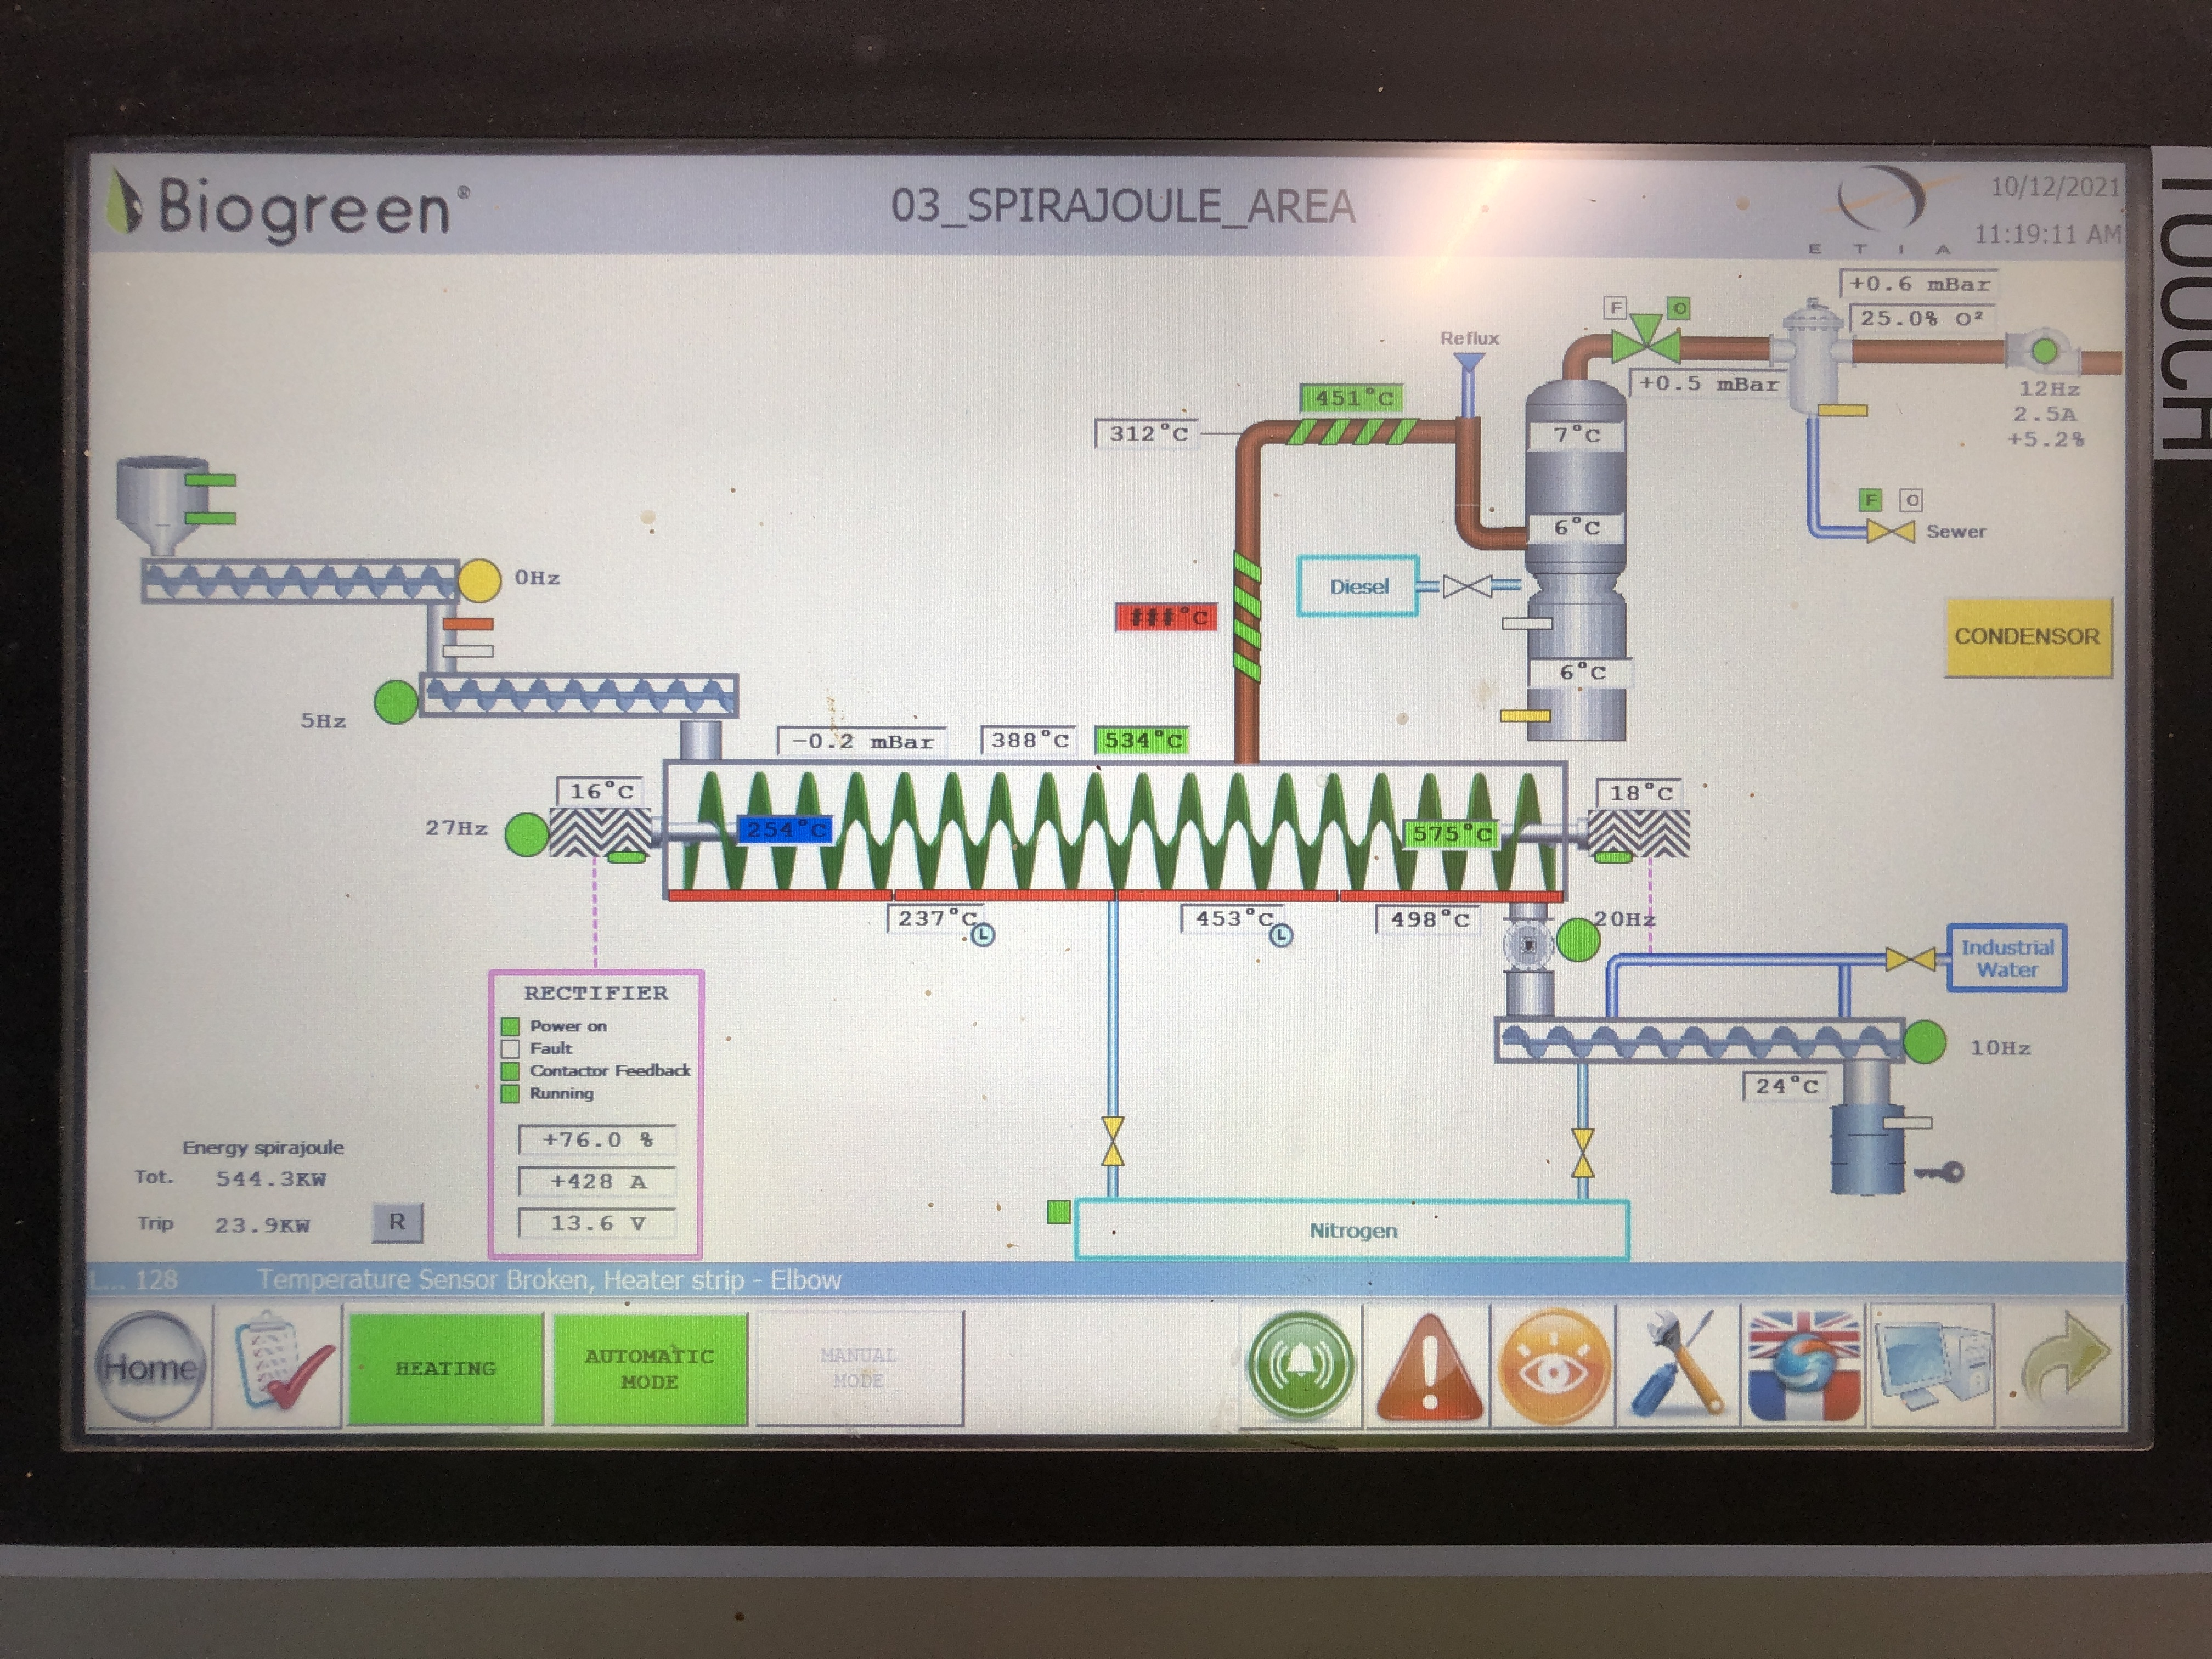
\includegraphics[width=0.7\linewidth,scale=0.7]{Bilder/Pyrolysis/Screen.png}
    \caption{Screen that displays monitoring of temperatures along the pyrolysis system developed by Biogreen\textsuperscript{\textregistered}.}
    \label{appFig:screen}
\end{figure}
\chapter{Sorption isotherm setup}\label{appSec:IsothermSetup}
In the following section, raw data for PFCA standard concentration calculations, mass of biochar weighed for each batch test, and pipetting volume are presented.

\begin{table}[h]
\centering
\caption{Concentration of first PFCA standard solution in 10 mL volumetric flasks accounted for purity of the PFCAs produced by Merck.}
\label{appTab:purityMass}
\begin{tabular}{lllll}
\toprule
Compound & Mass PFCA (g) & Purity (\%) & Mass PFCA (g) & {[}PFCA{]} (g/L) \\ 
& weighed & & accounted for purity & in   10 mL MeOH \\ \midrule
PFPeA & 0.0666 & 97 & 0.0646 & 6.46 \\
PFHxA & 0.0244 & 97 & 0.0237 & 2.37 \\
PFHpA & 0.0560 & 99 & 0.0554 & 5.54 \\
PFOA & 0.0116 & 95 & 0.0110 & 1.10 \\
PFNA & 0.0153 & 97 & 0.0148 & 1.48 \\
PFDA & 0.0114 & 98 & 0.0112 & 1.12 \\ \bottomrule
\end{tabular}
\end{table}

\begin{table}
\centering
\caption{Expected concentration of PFCA standards based on weight of native PFCA and dilution calculations versus analytical concentration by LC-MS/MS.}
\label{appTab:expConc}
\adjustbox{max width=\textwidth}{%
\begin{tabular}{lrrrrr} \toprule
 & \multicolumn{1}{l}{Me-OH standard (g L\textsuperscript{-1})} & \multicolumn{1}{l}{C11 (\textmu g L\textsuperscript{-1})} & \multicolumn{1}{l}{C12 (\textmu g L\textsuperscript{-1})} & \multicolumn{1}{l}{C13 (\textmu g L\textsuperscript{-1})} & \multicolumn{1}{l}{Analytical conc. (\textmu g L\textsuperscript{-1}}\\ \midrule
PFPeA & 6.46 & 5 168 & 103 & 15.5 & \\
PFHxA & 2.37 & 14 201 & 284 & 20.7 & \\
PFHpA & 5.60 & 3 360 & 27 & 10.2 & \\
PFOA & 1.16 & 13 920 & 557 & 13.4 & \\
PFNA & 1.53 & 18 360 & 367 & 10.0 & \\
PFDA & 1.14 & 17 100 & 684 & 10.3 & \\ \bottomrule
\end{tabular}}
\end{table}

\begin{table}
\centering
\caption{Mass biochar from Clean Wood Chips (CWC) weighed for each sample (n=60) (0.1000 $\pm$ 0.0004 g, \textmu = 0.1006 g, CV = 0.4 $\%$) C1-10 refers to the ten spike-concentrations for each PFCA batch test.}
\label{appTab:CWCmass}
\adjustbox{max width=\textwidth}{%
\begin{tabular}{lllllllllll}
\toprule
 & \multicolumn{10}{c}{Mass (g)} \\ \cline{2-11}
Compound & C1 & C2 & C3 & C4 & C5 & C6 & C7 & C8 & C9 & C10 \\ \midrule
PFPeA & 0.1008 & 0.1007 & 0.1007 & 0.1009 & 0.1014 & 0.1013 & 0.1011 & 0.1004 & 0.1009 & 0.1004 \\
PFHxA & 0.1014 & 0.1007 & 0.1014 & 0.1006 & 0.1002 & 0.1004 & 0.1014 & 0.1007 & 0.1004 & 0.1000 \\
PFHpA & 0.1005 & 0.1010 & 0.1005 & 0.1004 & 0.1009 & 0.1005 & 0.1002 & 0.1006 & 0.1007 & 0.1006 \\
PFOA & 0.1007 & 0.1008 & 0.1005 & 0.1009 & 0.1009 & 0.1002 & 0.1005 & 0.1006 & 0.1006 & 0.1009 \\
PFNA & 0.1002 & 0.1005 & 0.1004 & 0.1008 & 0.1008 & 0.1003 & 0.1002 & 0.1006 & 0.1006 & 0.1002 \\
PFDA & 0.1003 & 0.1001 & 0.1001 & 0.1001 & 0.1001 & 0.1003 & 0.1000 & 0.1005 & 0.1007 & 0.1007 \\ \bottomrule
\end{tabular}}
\end{table}


\begin{table}
\centering
\caption{Mass biochar from Ullensaker Sludge (ULS) weighed for each sample (n=60) (0.1000 $\pm$ 0.0003 g, \textmu = 0.1004 g, CV = 0.3 $\%$) C1-10 refers to the ten spike-concentrations for each PFCA batch test.}
\label{appTab:ULSmass}
\adjustbox{max width=\textwidth}{%
\begin{tabular}{lllllllllll}
\toprule
 & \multicolumn{10}{c}{Mass (g)} \\ \cline{2-11}
Compound & C1 & C2 & C3 & C4 & C5 & C6 & C7 & C8 & C9 & C10 \\ \midrule
PFPeA & 0.1007 & 0.1003 & 0.1004 & 0.1009 & 0.1009 & 0.1004 & 0.1009 & 0.1003 & 0.1000 & 0.1002 \\
PFHxA & 0.1009 & 0.1009 & 0.1003 & 0.1010 & 0.1002 & 0.1001 & 0.1006 & 0.1001 & 0.1000 & 0.1005 \\
PFHpA & 0.1001 & 0.1005 & 0.1004 & 0.1000 & 0.1004 & 0.1003 & 0.1005 & 0.1009 & 0.1005 & 0.1004 \\
PFOA & 0.1007 & 0.1000 & 0.1001 & 0.1009 & 0.1000 & 0.1001 & 0.1005 & 0.1001 & 0.1000 & 0.1002 \\
PFNA & 0.1001 & 0.1000 & 0.1000 & 0.1006 & 0.1000 & 0.1006 & 0.1005 & 0.1007 & 0.1007 & 0.1006 \\
PFDA & 0.1005 & 0.1005 & 0.1001 & 0.1008 & 0.1005 & 0.1001 & 0.1004 & 0.1002 & 0.1000 & 0.1003 \\ \bottomrule
\end{tabular}}
\end{table}

\begin{table}
\centering
\caption{Mass biochar from Biorest Lindum (BRL) weighed for each sample (n=60) (0.1000 $\pm$ 0.0003 g, \textmu = 0.1005 g, CV = 0.3 $\%$) C1-10 refers to the ten spike-concentrations for each PFCA batch test.}
\label{appTab:BRLmass}
\adjustbox{max width=\textwidth}{%
\begin{tabular}{lllllllllll}
\toprule
 & \multicolumn{10}{c}{Mass (g)} \\ \cline{2-11}
Compound & C1 & C2 & C3 & C4 & C5 & C6 & C7 & C8 & C9 & C10 \\ \midrule
PFPeA & 0.1003 & 0.1006 & 0.1000 & 0.1005 & 0.1007 & 0.1009 & 0.1005 & 0.1006 & 0.1007 & 0.1007 \\
PFHxA & 0.1003 & 0.1008 & 0.1004 & 0.0999 & 0.1004 & 0.1001 & 0.1002 & 0.1002 & 0.1007 & 0.1004 \\
PFHpA & 0.1005 & 0.1009 & 0.1010 & 0.1000 & 0.1006 & 0.1007 & 0.1007 & 0.1003 & 0.1005 & 0.1004 \\
PFOA & 0.1006 & 0.1008 & 0.1009 & 0.1002 & 0.1004 & 0.1002 & 0.1006 & 0.1001 & 0.1001 & 0.1000 \\
PFNA & 0.1010 & 0.1009 & 0.1010 & 0.1003 & 0.1002 & 0.0999 & 0.1005 & 0.1010 & 0.1005 & 0.1008 \\
PFDA & 0.1001 & 0.1007 & 0.1003 & 0.1010 & 0.1006 & 0.1008 & 0.1008 & 0.1001 & 0.1010 & 0.1004 \\ \bottomrule
\end{tabular}}
\end{table}

\begin{table}
\centering
\caption{Volume pipetted from working standards using different combinations of micro- (5-50 {\textmu}l and 200-1000 {\textmu}l) and milli pipettes (2-10 mL).}
\label{appTab:pipetting}
\adjustbox{max width=\textwidth}{%
\begin{tabular}{lrrrrrrrrrr} \toprule
\multicolumn{1}{c}{\textbf{}} & \multicolumn{10}{c}{Pipetting   volume (mL) from C11 (white) and C12 (grey)} \\ \cline{2-11} 
Compound & V1 & V2 & V3 & V4 & V5 & V6 & V7 & V8 & V9 & V10 \\ \midrule
PFPeA & \cellcolor[HTML]{C0C0C0}0.0145 & 0.314 & 0.653 & 0.967 & 1.305 & 1.620 & 1.935 & 2.274 & 2.900 & 2.902 \\
PFHxA & \cellcolor[HTML]{C0C0C0}0.0105 & 0.238 & 0.467 & 0.705 & 0.933 & 1.180 & 1.408 & 1.637 & 1.866 & 2.113 \\
PFHpA & \cellcolor[HTML]{C0C0C0}0.0240 & \cellcolor[HTML]{C0C0C0}23.250 & 0.410 & 0.632 & 0.855 & 1.079 & 1.302 & 1.525 & 1.749 & 1.935 \\
PFOA & \cellcolor[HTML]{C0C0C0}0.0110 & 0.475 & 0.960 & 1.437 & 1.922 & 2.398 & 2.874 & 3.360 & 3.843 & 4.310 \\
PFNA & \cellcolor[HTML]{C0C0C0}0.0220 & 0.483 & 0.967 & 1.457 & 1.935 & 2.425 & 2.915 & 3.390 & 3.880 & 4.357 \\
PFDA & \cellcolor[HTML]{C0C0C0}0.0365 & 1.623 & 3.245 & 4.868 & 6.490 & 8.115 & 9.737 & 11.360 & 12.982 & 14.620 \\ \bottomrule
\end{tabular}}
\end{table}

\begin{table}
\centering
\caption{Mass for each PFCA batch test prepared in 50 mL PP Falcon tubes, assuming a density of water of 1 g/mL (50.0000 $\pm$ 0.02 mL, \textmu = 50.0075 mL, CV=0.04$\%$).}
\label{appTab:milliQ}
\adjustbox{max width=\textwidth}{%
\begin{tabular}{lllllllllll} \toprule
 & \multicolumn{10}{c}{Mass (g) water weighed} \\ \cline{2-11}
Compound & V1 & V2 & V3 & V4 & V5 & V6 & V7 & V8 & V9 & V10 \\ \midrule
PFPeA & 50.0129 & 50.0108 & 50.0016 & 50.0020 & 49.9934 & 50.0001 & 50.0072 & 49.9916 & 49.9902 & 49.9943 \\
PFHxA & 50.0059 & 50.0262 & 49.9934 & 50.0107 & 50.0093 & 49.9938 & 49.9971 & 50.0015 & 50.0062 & 50.0001 \\
PFHpA & 50.0123 & 50.0084 & 50.0005 & 50.1474 & 49.9976 & 50.0055 & 49.9948 & 50.0037 & 50.0165 & 49.9950 \\
PFOA & 50.0095 & 50.0092 & 50.0128 & 49.9976 & 50.0055 & 50.0053 & 50.0036 & 50.0143 & 50.0090 & 49.9940 \\
PFNA & 50.0149 & 50.0030 & 49.9966 & 50.0463 & 50.0070 & 49.9856 & 50.0024 & 50.0062 & 50.0161 & 50.0445 \\
PFDA & 50.0120 & 50.0021 & 50.0035 & 50.0068 & 49.9963 & 50.0120 & 49.9984 & 49.9892 & 50.0101 & 50.0081 \\ \bottomrule
\end{tabular}}
\end{table}

Soil composition
\chapter{LC-MS/MS}\label{appSec:LCMS}

\begin{table}
\centering
\caption{Gradient between the two mobile phases used during UPLC-MS/MS. Water phase (A): Milli-Q water with 2 mM ammonium acetate, organic phase (B): pure MeOH. Run time = 6 min.}
\label{apptab:gradient}
\begin{tabular}{ccccc} \toprule
\multicolumn{1}{l}{\textbf{Time (min)}} & \multicolumn{1}{l}{\textbf{Flow}} & \multicolumn{1}{l}{\textbf{\% A}} & \multicolumn{1}{l}{\textbf{\% B}} & \multicolumn{1}{l}{\textbf{Step}} \\ \midrule
0 & 0.25 & 80 & 20 & Init \\
0.1 & 0.25 & 80 & 20 & 6 \\
0.2 & 0.25 & 50 & 50 & 6 \\
0.8 & 0.25 & 30 & 70 & 6 \\
1.5 & 0.25 & 20 & 80 & 6 \\
2.8 & 0.25 & 15 & 85 & 5 \\
4.5 & 0.25 & 0 & 100 & 6 \\
5.5 & 0.25 & 0 & 100 & 6 \\
5.6 & 0.25 & 80 & 20 & 6 \\
6 & 0.25 & 80 & 20 & 6 \\ \bottomrule
\end{tabular}
\end{table}

\begin{table}
\centering
\caption{Tune parameters for UPLC-Xevo TQS instrument.}
\label{apptab:tune}
\begin{tabular}{ll} \toprule
\multicolumn{1}{c}{\textbf{ESI (-)}} &  \\ \midrule
Capillary (kV) & 2 \\
Cone (V) & 25 \\
Source Offset (V) & 40 \\
Desolvation temperature   (\textdegree C) & 450 \\
Desolvation Gas flow   (L/h) & 650 \\
Cone (L/h) & 150 \\
Nebuliszer (Bar) & 6 \\
Source Temperature (\textdegree C) & 150 \\ \bottomrule
\end{tabular}
\end{table}

\begin{figure}
    \centering
    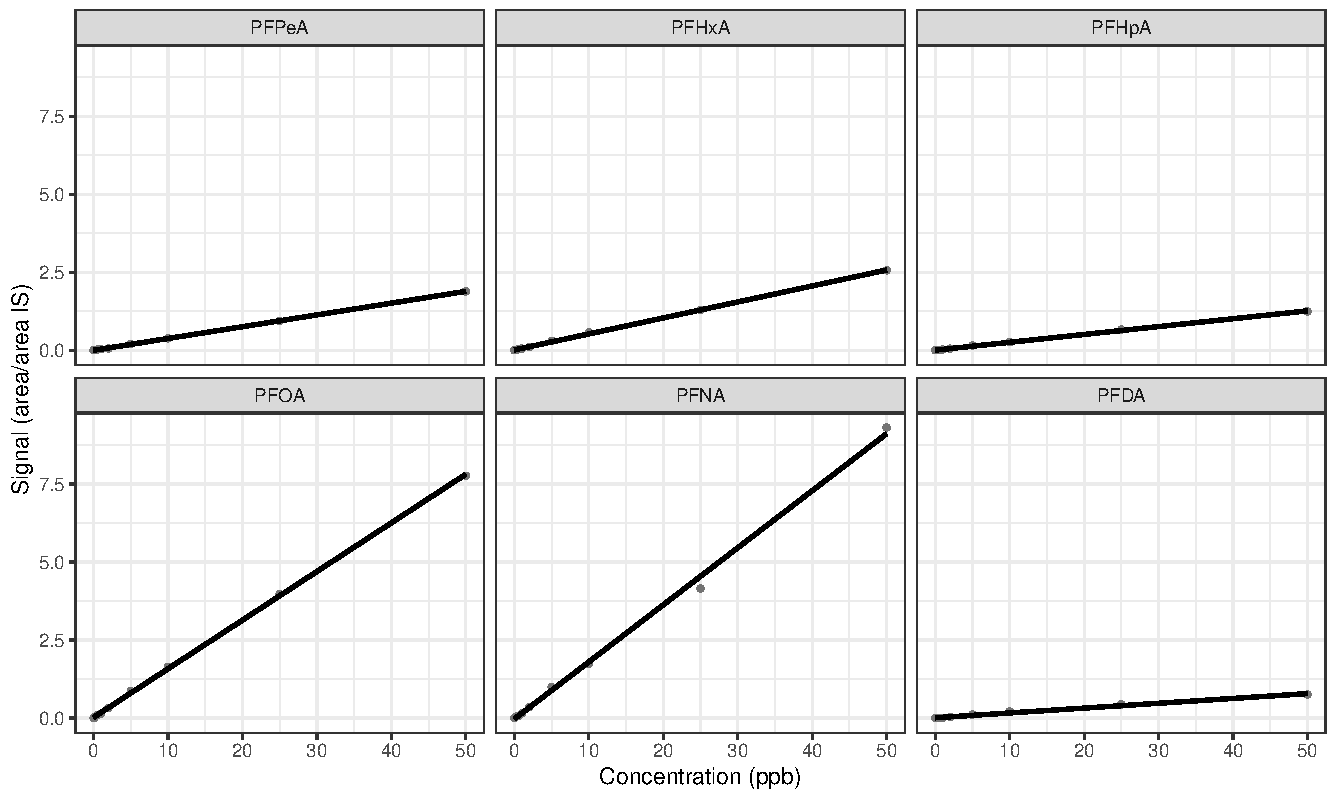
\includegraphics[width=\textwidth]{R/figs/CC_all.pdf}
    \caption{Calibration curve solvent blank}
    \label{appfig:CC}
\end{figure}

Matrix effect

\begin{figure}
    \centering
    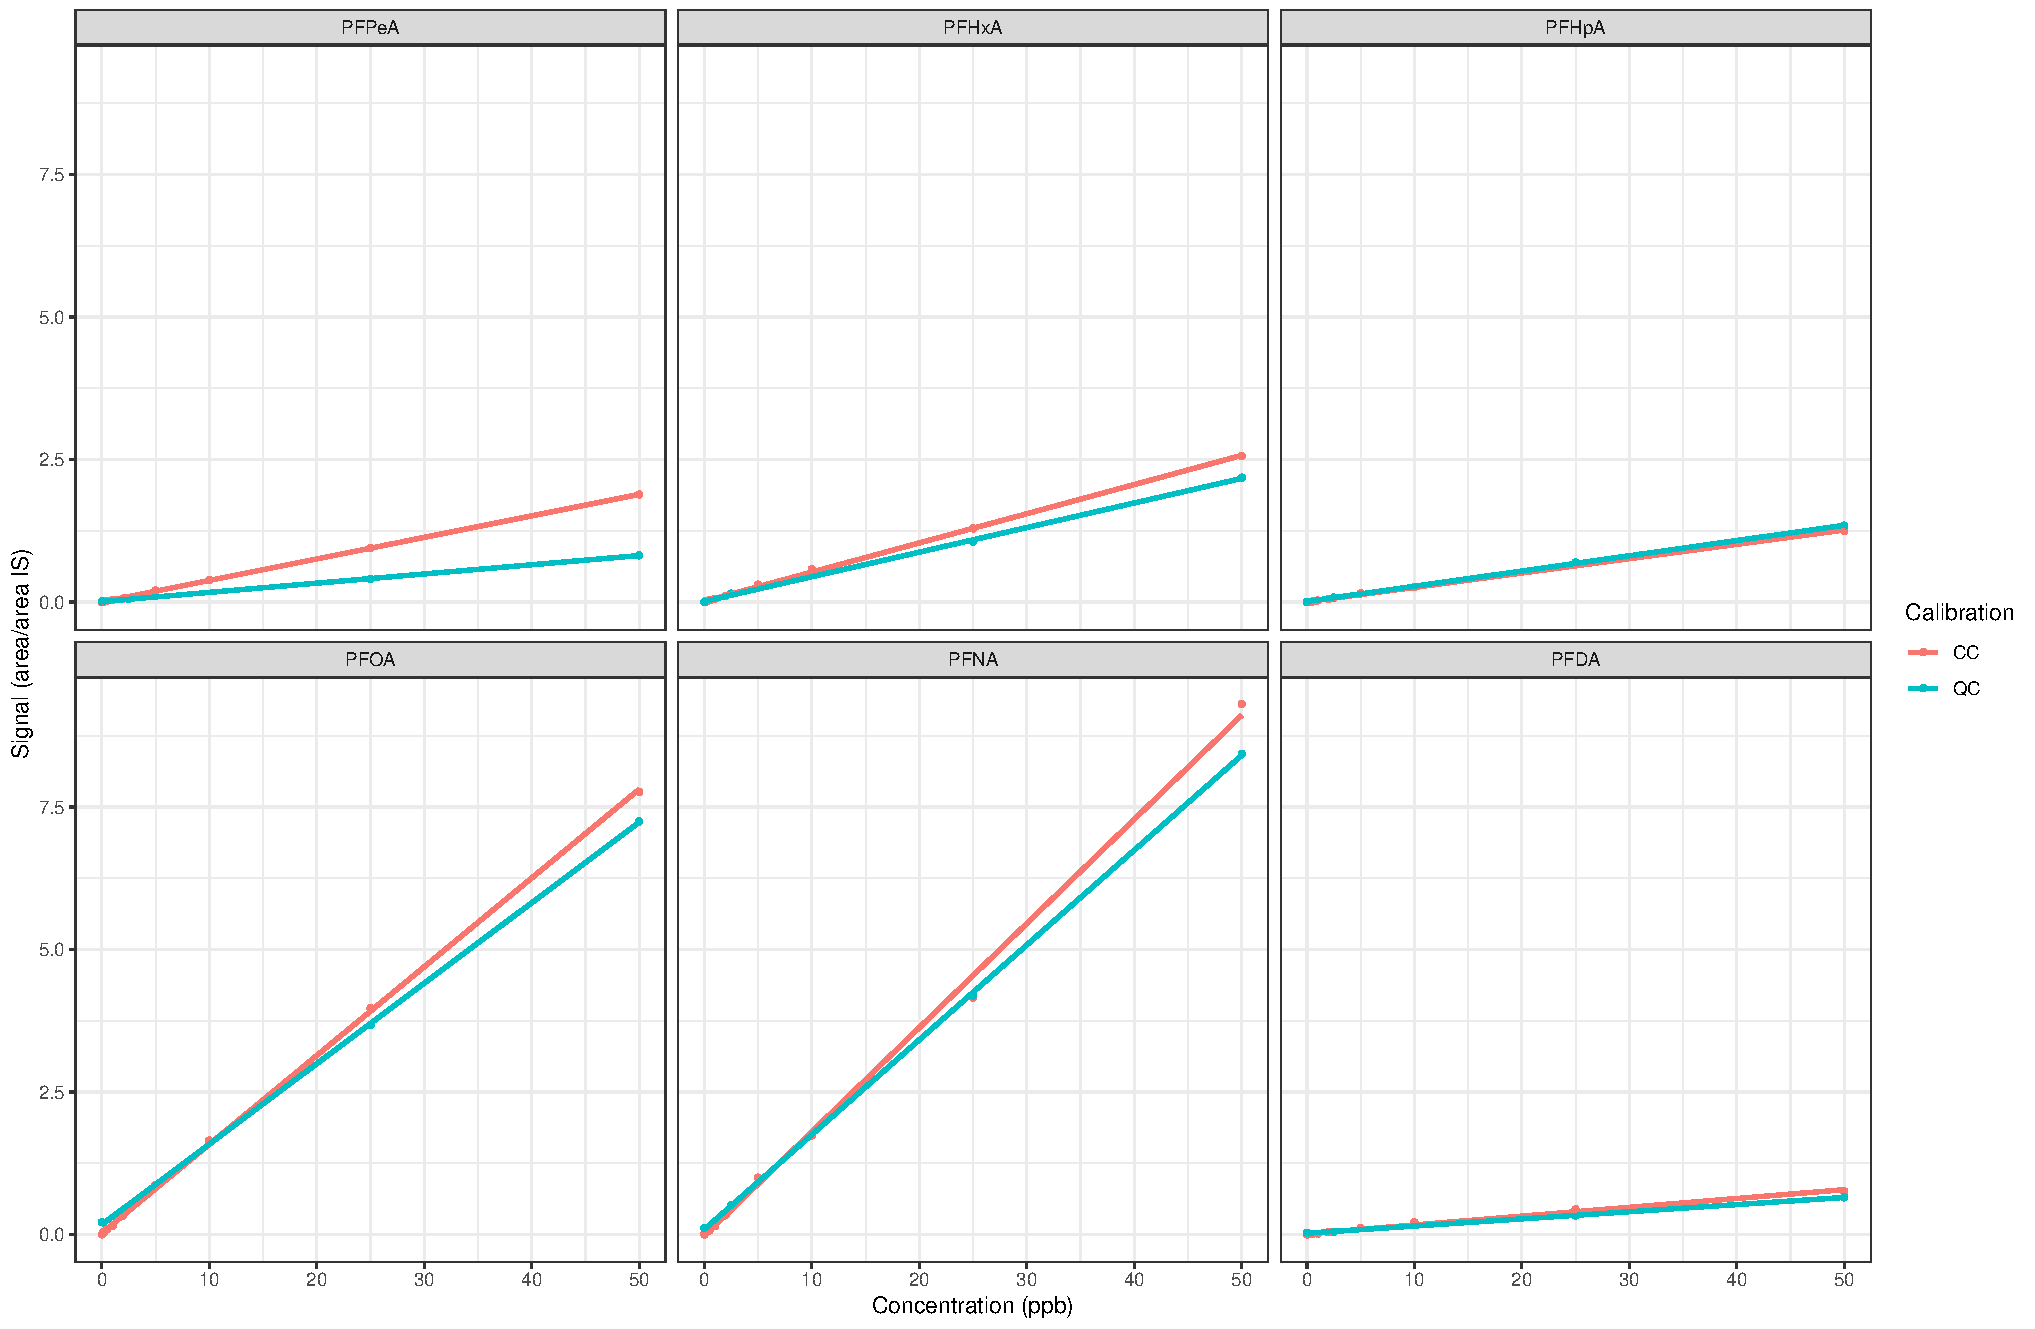
\includegraphics[width=\textwidth]{R/figs/CCQC_matrixeffect.pdf}
    \caption{Matrix effect (ME) for the PFCAs where CC = calibration curve in solvent blank, QC = matrix matched calibration curve. QC in line with CC indicates no ME, QC \textgreater CC = ion enhancement, CC \textless QC = ion suppression.}
    \label{appfig:ME}
\end{figure}
\chapter{Miscellaneous laboratory tests}\label{appSec:misclab}

In the following section, miscellaneous laboratory performed to strengthen the experimental certainty of the batch sorption isotherm tests are presented. 

\subsection{pH and conductivity}

\begin{figure} 
\centering
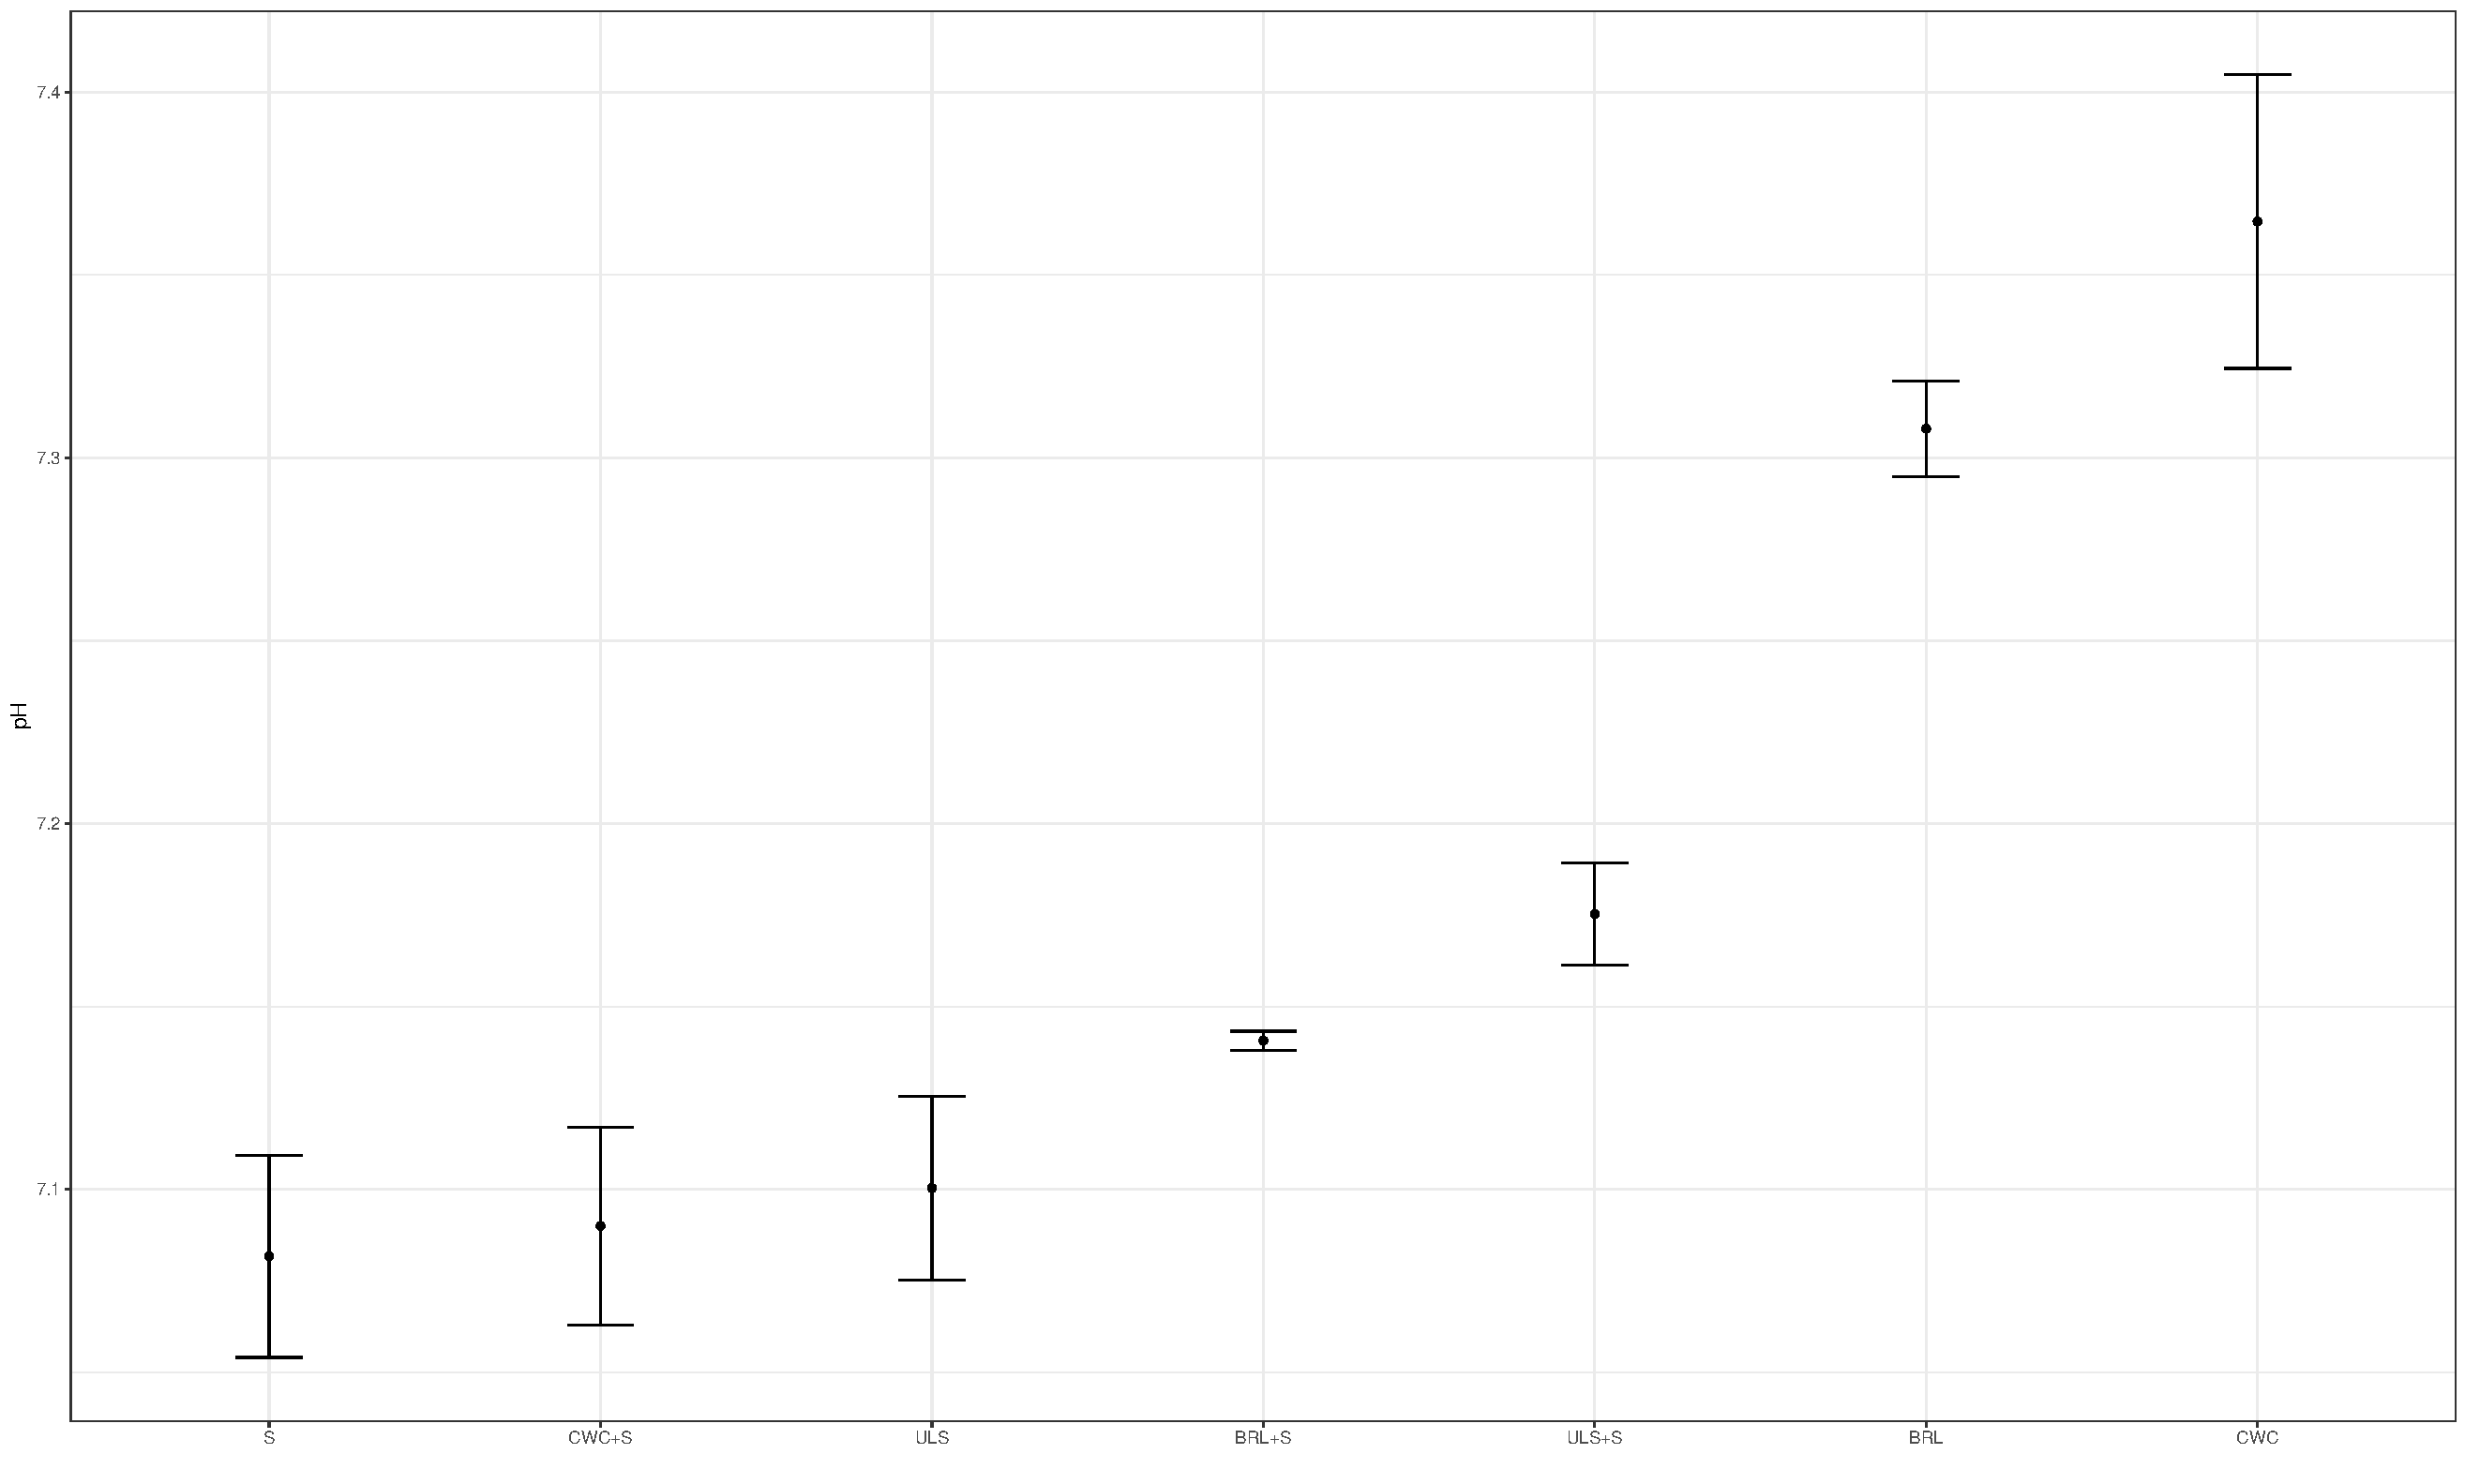
\includegraphics[width=\textwidth]{R/figs/pH.pdf}
\caption{Plot of pH measurements for 50 mL milli-Q water batch tests with 0.1 g biochars (CWC, ULS, BRL) and 5 g soil (S) (n=3).}
\label{appfig:pH}
\end{figure}

\begin{figure} 
\centering
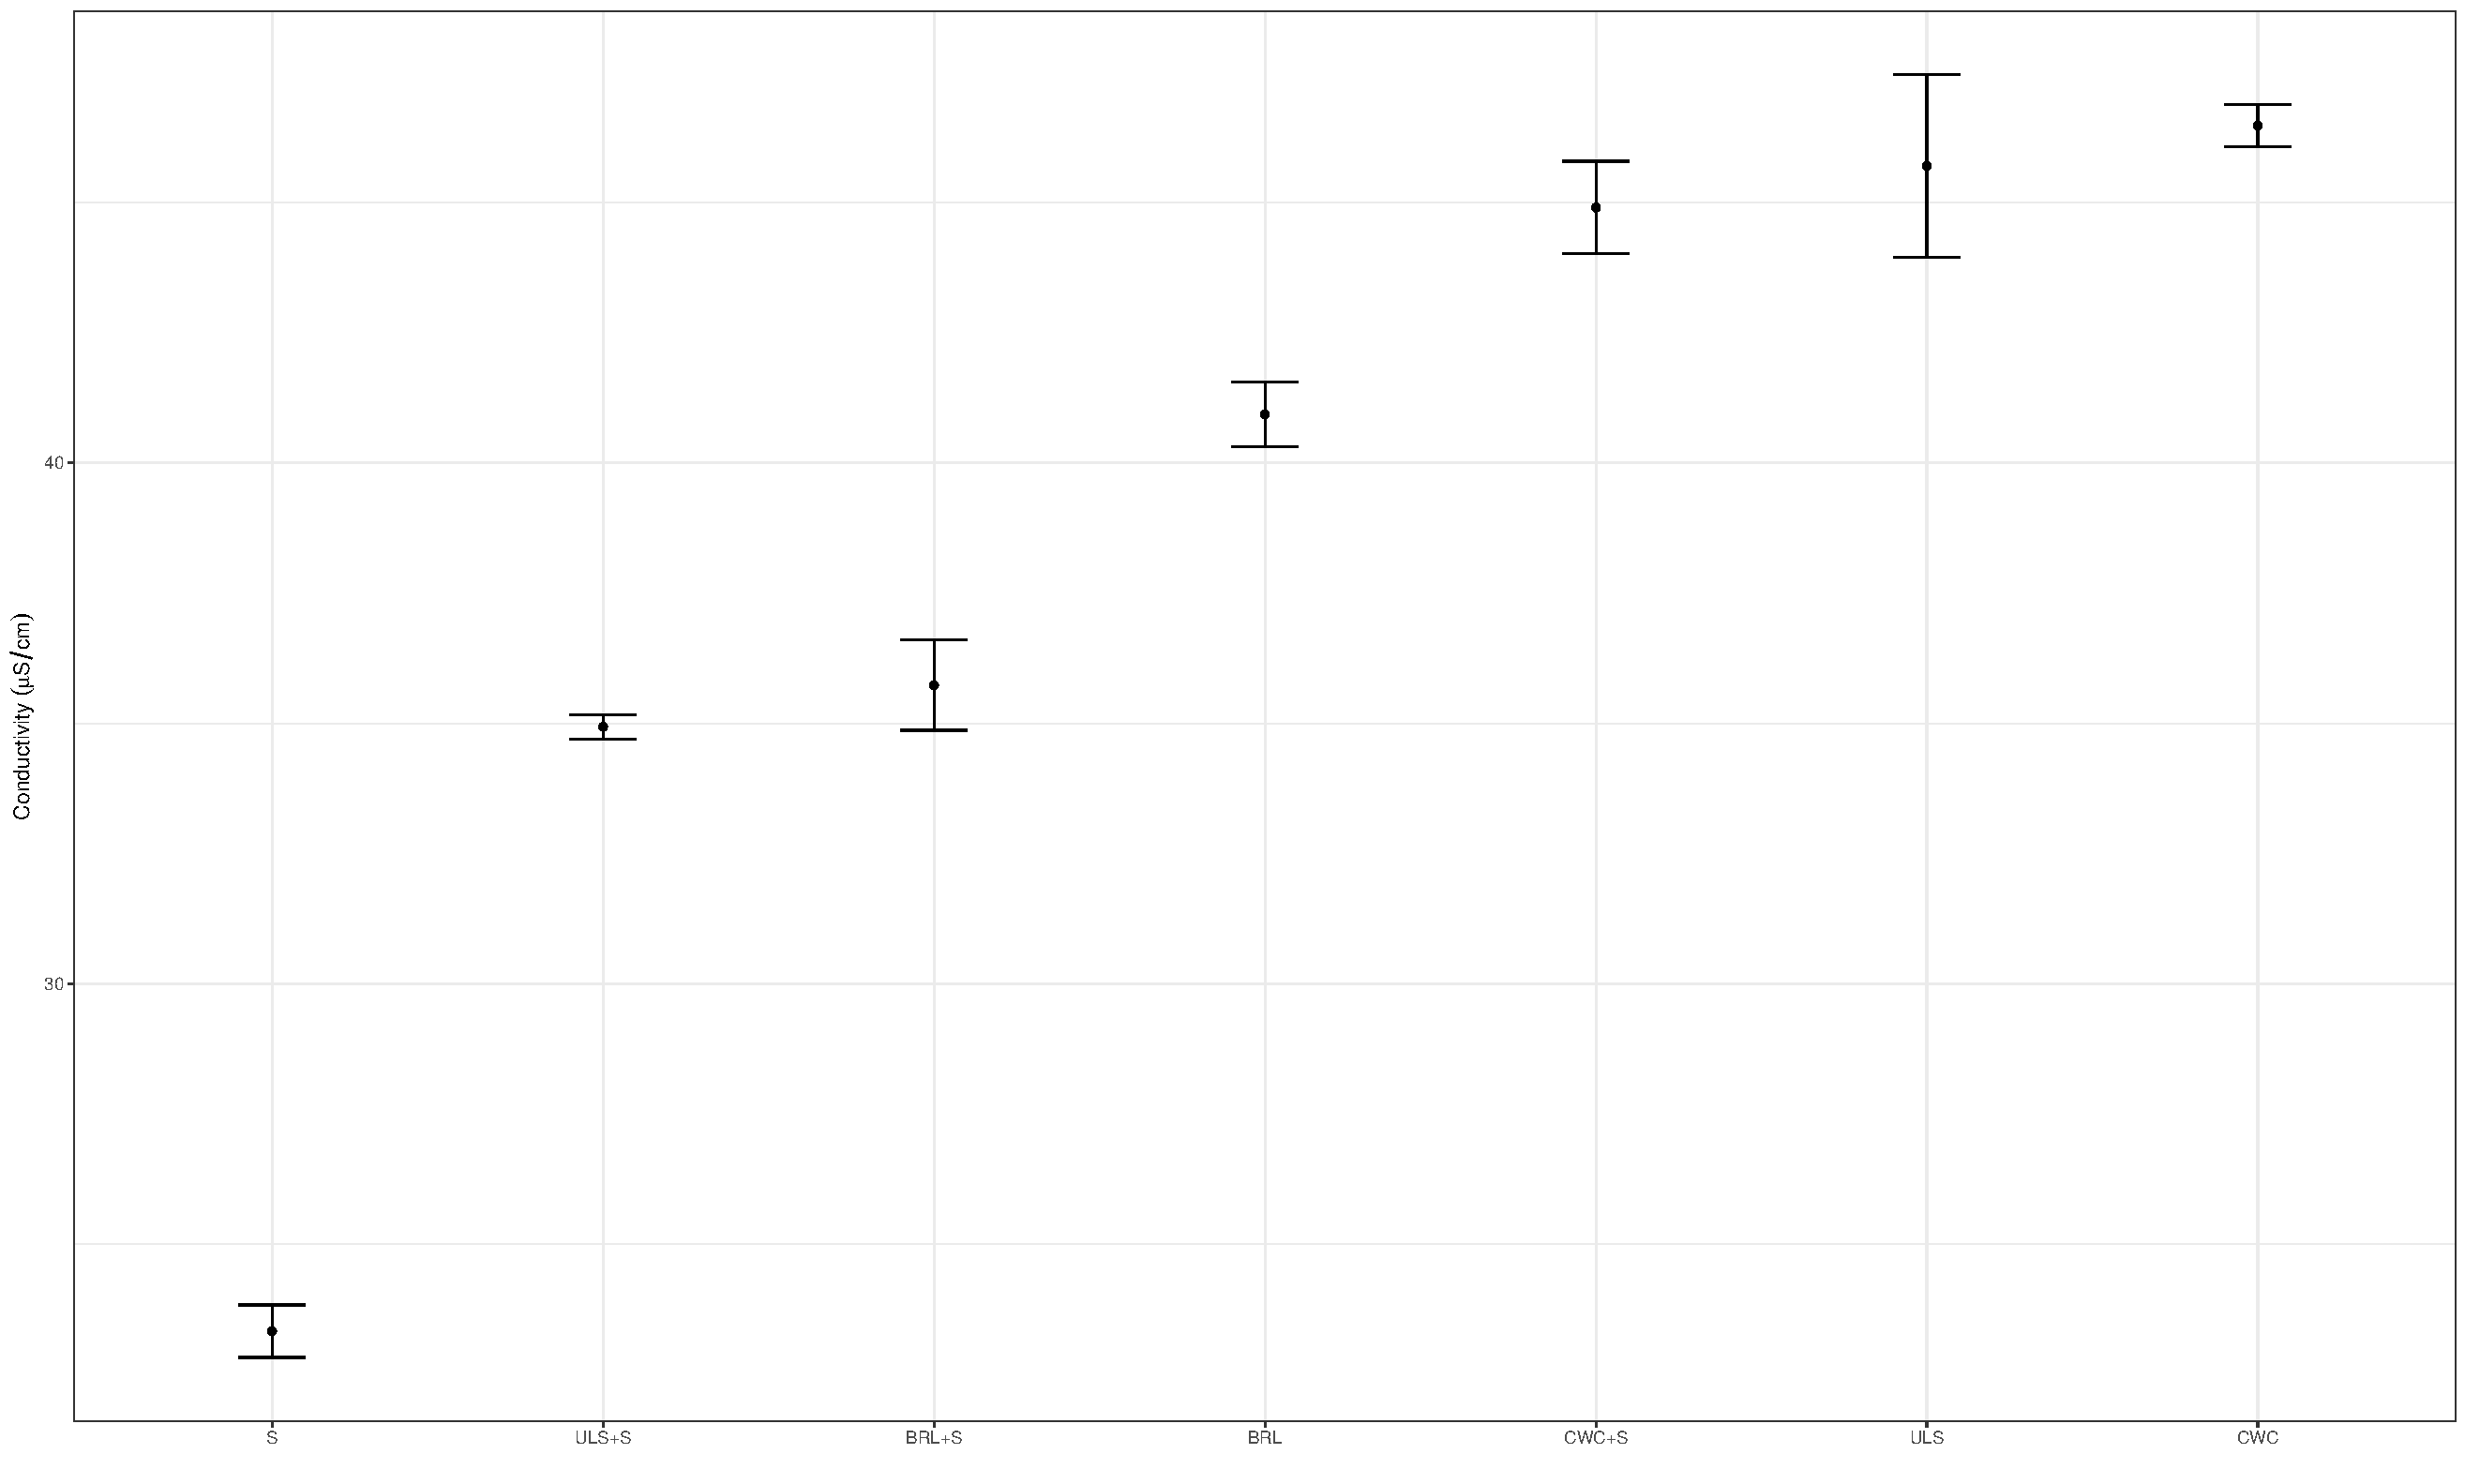
\includegraphics[width=\textwidth]{R/figs/conductivity.pdf}
\caption{Plot of conductivity measurements for 50 mL milli-Q water batch tests with 0.1 g biochars (CWC, ULS, BRL) and 5 g soil (S) (n=3).}
\label{appfig:cond}
\end{figure}

\begin{table}[h]
\centering
\caption{Pipette calibration for 2-10 mL pipette. PASS is given if CV $\leq$ 1.0 \% and the average volume dispensed is within 1.8400 - 2.1600 mL. }
\label{appTab:pip2-10}
\adjustbox{max width=\textwidth}{%
\begin{tabular}{lrrrrrrr} \toprule
 & \multicolumn{1}{l}{} &  &  &  & \multicolumn{3}{r}{Operator: Thermo Fishcer Scientific} \\
 & \multicolumn{1}{l}{} &  &  &  & \multicolumn{3}{r}{Serial number: EJ08813} \\
 & \multicolumn{1}{l}{} &  &  &  & \multicolumn{3}{r}{Date: 04.10.2021} \\ \midrule
\multicolumn{1}{c}{\textbf{\begin{tabular}[c]{@{}c@{}}Test volume\\ (mL)\end{tabular}}} & \multicolumn{1}{c}{\textbf{}} & \multicolumn{1}{c}{\textbf{\begin{tabular}[c]{@{}c@{}}Weight of\\ dispensed\\ volume (g)\end{tabular}}} & \multicolumn{1}{c}{\textbf{\begin{tabular}[c]{@{}c@{}}Corrected\\ volume (g)\end{tabular}}} & \multicolumn{1}{c}{\textbf{\begin{tabular}[c]{@{}c@{}}Average\\ volume (mL)\end{tabular}}} & \multicolumn{1}{c}{\textbf{SDEV}} & \multicolumn{1}{c}{\textbf{CV}} & \multicolumn{1}{c}{\textbf{PASS/FAIL}} \\ \midrule
\multicolumn{1}{c}{\textbf{2}} & \multicolumn{1}{c}{\textbf{}} &  &  & 2.0868 & 0.006 & 0.3 \% &  \\
\multicolumn{1}{c}{\textbf{}} & 1 & 2.0804 & 2.0842 &  &  &  &  \\
 & 2 & 2.0923 & 2.0961 &  &  &  &  \\
 & 3 & 2.0902 & 2.0940 &  &  &  &  \\
 & 4 & 2.0861 & 2.0899 &  &  &  &  \\
 & 5 & 2.0817 & 2.0855 &  &  &  &  \\
 & 6 & 2.0852 & 2.0890 &  &  &  &  \\
 & 7 & 2.0807 & 2.0845 &  &  &  &  \\
 & 8 & 2.0829 & 2.0867 &  &  &  &  \\
 & 9 & 2.0778 & 2.0815 &  &  &  & \textbf{} \\
 & 10 & 2.0727 & 2.0764 &  &  &  &  \\
 & \multicolumn{1}{l}{} &  &  & \textbf{} & \textbf{} &  & \cellcolor[HTML]{C0C0C0}\textbf{PASS} \\ \bottomrule
\end{tabular}}
\end{table}



\begin{table}
\centering
\caption{Pipette calibration for 200-1000 μL pipette. PASS is given if CV $\leq$ 1.0 \% and the average volume dispensed is within 992 - 1008 μL. }
\label{appTab:pip200-1000}
\adjustbox{max width=\textwidth}{%
\begin{tabular}{lrrrrrrr} \toprule
 & \multicolumn{1}{l}{} & \multicolumn{1}{l}{} & \multicolumn{1}{l}{} & \multicolumn{1}{l}{} & \multicolumn{3}{r}{Operator: Thermo Fischer Scientific} \\
 & \multicolumn{1}{l}{} & \multicolumn{1}{l}{} & \multicolumn{1}{l}{} & \multicolumn{1}{l}{} & \multicolumn{3}{r}{Serial Number: EH23798 4500} \\
 & \multicolumn{1}{l}{} & \multicolumn{1}{l}{} & \multicolumn{1}{l}{} & \multicolumn{1}{l}{} & \multicolumn{3}{r}{Date: 04.10.2021} \\ \midrule
\multicolumn{1}{c}{\textbf{\begin{tabular}[c]{@{}c@{}}Test volume \\ (μL)\end{tabular}}} & \textbf{} & \multicolumn{1}{c}{\textbf{\begin{tabular}[c]{@{}c@{}}Weight of\\ dispensed\\ volume (g)\end{tabular}}} & \multicolumn{1}{c}{\textbf{\begin{tabular}[c]{@{}c@{}}Corrected\\ volume (μL)\end{tabular}}} & \multicolumn{1}{c}{\textbf{\begin{tabular}[c]{@{}c@{}}Average\\ volume (μL)\end{tabular}}} & \multicolumn{1}{c}{\textbf{SDEV}} & \multicolumn{1}{c}{\textbf{CV}} & \multicolumn{1}{c}{\textbf{PASS/FAIL}} \\ \midrule
\multicolumn{1}{c}{\textbf{1000}} & \textbf{} & \multicolumn{1}{l}{} & \multicolumn{1}{l}{} & 994.2 & 5 & 0.5 \% & \multicolumn{1}{l}{} \\
\multicolumn{1}{c}{} & 1 & 997.0 & 998.8 &  &  &  &  \\
 & 2 & 999.4 & 1001.2 &  &  &  &  \\
 & 3 & 990.4 & 992.2 &  &  &  &  \\
 & 4 & 992.3 & 994.1 &  &  &  &  \\
 & 5 & 990.5 & 992.3 &  &  &  &  \\
 & 6 & 990.9 & 992.7 &  &  &  &  \\
 & 7 & 983.8 & 985.6 &  &  &  &  \\
 & 8 & 990.9 & 992.7 &  &  &  &  \\
 & 9 & 990.5 & 992.3 &  &  &  &  \\
 & 10 & 998.4 & 1000.2 &  &  &  &  \\
 & \multicolumn{1}{l}{} & \multicolumn{1}{l}{} & \multicolumn{1}{l}{} & \multicolumn{1}{l}{\textbf{}} & \multicolumn{1}{l}{\textbf{}} & \multicolumn{1}{l}{} & \multicolumn{1}{l}{\cellcolor[HTML]{C0C0C0}\textbf{PASS}} \\ \bottomrule
\end{tabular}}
\end{table}


\begin{table}
\centering
\caption{Pipette calibration for 5 - 50 μL pipette. PASS is given if CV $\leq$ 2.5 \% and the average volume dispensed is within 19.8 - 20.2 μL. }
\label{appTab:pip5-50}
\adjustbox{max width=\textwidth}{%
\begin{tabular}{lrrrrrrr} \toprule
 & \multicolumn{1}{l}{} & \multicolumn{1}{l}{} & \multicolumn{1}{l}{} & \multicolumn{1}{l}{} & \multicolumn{3}{r}{Operator: Thermo Fischer Scientific} \\
 & \multicolumn{1}{l}{} & \multicolumn{1}{l}{} & \multicolumn{1}{l}{} & \multicolumn{1}{l}{} & \multicolumn{3}{r}{Serial Number: EH94947 4500} \\
 & \multicolumn{1}{l}{} & \multicolumn{1}{l}{} & \multicolumn{1}{l}{} & \multicolumn{1}{l}{} & \multicolumn{3}{r}{Date: 04.10.2021} \\ \midrule
\multicolumn{1}{c}{\textbf{\begin{tabular}[c]{@{}c@{}}Test volume\\ (μL)\end{tabular}}} & \multicolumn{1}{c}{\textbf{}} & \multicolumn{1}{c}{\textbf{\begin{tabular}[c]{@{}c@{}}Weight of\\ dispensed\\ volume (g)\end{tabular}}} & \multicolumn{1}{c}{\textbf{\begin{tabular}[c]{@{}c@{}}Corrected\\ volume (mL)\end{tabular}}} & \multicolumn{1}{c}{\textbf{\begin{tabular}[c]{@{}c@{}}Average\\ volume (mL)\end{tabular}}} & \multicolumn{1}{c}{\textbf{SDEV}} & \multicolumn{1}{c}{\textbf{CV}} & \multicolumn{1}{c}{\textbf{PASS/FAIL}} \\ \midrule
\multicolumn{1}{c}{\textbf{20}} & &  &  & 19.8 & 0.4 & 2 $\%$ & \multicolumn{1}{l}{} \\
 & 1 & 19.8 & 19.8 &  &  &  &  \\
 & 2 & 19.5 & 19.5 &  &  &  &  \\
 & 3 & 19.8 & 19.8 &  &  &  &  \\
 & 4 & 20.8 & 20.8 &  &  &  &  \\
 & 5 & 19.9 & 19.9 &  &  &  &  \\
 & 6 & 19.6 & 19.6 &  &  &  &  \\
 & 7 & 19.7 & 19.7 &  &  &  &  \\
 & 8 & 19.5 & 19.5 &  &  &  &  \\
 & 9 & 19.2 & 19.2 &  &  &  &  \\
 & 10 & 19.9 & 19.9 &  &  &  & \cellcolor[HTML]{FFFFFF}\textbf{} \\
 & \multicolumn{1}{l}{} & \multicolumn{1}{l}{} & \multicolumn{1}{l}{} &  &  &  & \multicolumn{1}{l}{\cellcolor[HTML]{C0C0C0}\textbf{PASS}} \\ \bottomrule
\end{tabular}}
\end{table}

\begin{table}
\centering
\caption{Volume calibration for 50 mL Falcon high-clarity polypropylene (PP) conical centrifuge tube. PASS is given if CV $\leq$ and the average volume filled is within 49.0 - 51.0 mL.}
\label{appTab:PPcentrifuge}
\adjustbox{max width=\textwidth}{%
\begin{tabular}{crrrrrrrr} \toprule
 &  &  &  &  & \multicolumn{4}{r}{Date: 26.10.2021} \\ \midrule
\multicolumn{1}{c}{\textbf{\begin{tabular}[c]{@{}c@{}}Test\\volume (mL)\end{tabular}}} & \multicolumn{1}{c}{\textbf{}} & \multicolumn{1}{c}{\textbf{\begin{tabular}[c]{@{}c@{}}Initial \\ weight  (g)\end{tabular}}} & \multicolumn{1}{c}{\textbf{\begin{tabular}[c]{@{}c@{}}Final\\weight (g)\end{tabular}}} & \multicolumn{1}{c}{\textbf{\begin{tabular}[c]{@{}c@{}}Net \\weight (g)\end{tabular}}} & \multicolumn{1}{c}{\textbf{\begin{tabular}[c]{@{}c@{}}Average \\ volume (mL)\end{tabular}}} & \multicolumn{1}{c}{\textbf{SDEV}} & \multicolumn{1}{c}{\textbf{CV}} & \multicolumn{1}{c}{\textbf{PASS/FAIL}} \\ \midrule
\textbf{50} &  &  &  &  & 48.4756 & 0.2 & 0.4 \% &  \\
 & 1 & 13.0354 & 61.3521 & 48.3167 &  &  &  &  \\
 & 2 & 13.0572 & 61.3498 & 48.2926 &  &  &  &  \\
 & 3 & 13.0154 & 61.1161 & 48.1007 &  &  &  &  \\
 & 4 & 13.0857 & 61.8386 & 48.7529 &  &  &  &  \\
 & 5 & 13.0658 & 61.6241 & 48.5583 &  &  &  &  \\
 & 6 & 12.9908 & 61.6972 & 48.7064 &  &  &  &  \\
 & 7 & 13.0073 & 61.4474 & 48.4401 &  &  &  &  \\
 & 8 & 13.0699 & 61.7248 & 48.6549 &  &  &  &  \\
 & 9 & 12.7855 & 61.3788 & 48.5933 &  &  &  &  \\
 & 10 & 12.9962 & 61.3365 & 48.3403 &  &  &  &  \\
 &  &  &  &  &  &  &  & \multicolumn{1}{l}{\cellcolor[HTML]{C0C0C0}\textbf{FAIL}} \\ \bottomrule
\end{tabular}}
\end{table}

\begin{table}
\centering
\caption{Mass CWC left in syringe after filtering of biochar-PFCA solution. Total mass CWC is 0.1000 $\pm$ 0.004 g.}
\label{appTab:CWCloss}
\begin{tabular}{rrrrr} \toprule
 & Mass (g) & \multicolumn{1}{c}{$\bar{x}$} & \multicolumn{1}{c}{SDEV} & \multicolumn{1}{c}{CV}  \\ \midrule
 & & 0.0488 & 0.003 & 8 $\%$ \\
1 & 0.0429 \\
2 & 0.0413 \\
3 & 0.0484 \\
4 & 0.0428 \\
5 & 0.0485 \\ \bottomrule
\end{tabular}
\end{table}

Here can include soil precipitation test?


\chapter{Element analysis soil and biochar}\label{appSec:elements}

\begin{table}
\centering
\caption{Total element composition of the biochars used in this thesis.}
\adjustbox{max width=\textwidth}{
\label{apptab:totelem}
\begin{threeparttable}
\begin{tabular}{lccccccc} 
\toprule
\textbf{}                   & \textbf{} & \multicolumn{2}{c}{\textbf{CWC}} & \multicolumn{2}{c}{\textbf{ULS}} & \multicolumn{2}{c}{\textbf{DSL}} \\ \cline{3-8} 
                                       &           & Mean              & Std.dev          & Mean             & Std.dev           & Mean            & Std.dev            \\ \hline \addlinespace
\textbf{Main elements} &&&&&&& \\ \hline \addlinespace
C                                       & \%        & 91.4              & 2.5              & 29.63            & 0.47              & 13.5            & 0.2                \\
N                                       & \%        & 0.69              & 0.02             & 1.131            & 0.039             & 0.82            & 0.02               \\
H                                       & \%        & 1.01              & 0.14             & 1.243            & 0.045             & 1.05            & 0.16               \\
O\textsuperscript{*}                            & \%        &     5.5              &                  &       57.1           &                   &        61.4         &                    \\
Ca                        & g/kg      & 8.0               & 0.2              & 21               &                   & 26.0            & 0.0                \\
Fe                        & g/kg      & 0.13              & 0.04             & 23               &                   & 180             & 0                  \\
K                         & g/kg      & 4.03              & 0.06             & 6.8              &                   & 3.7             & 0.1                \\
Mg                        & g/kg      & 0.91              & 0.02             & 5.3              &                   & 4.70            & 0.17               \\
Na                         & g/kg      & 0.05              & 0.00             & 2.4              &                   & 1.83            & 0.06               \\
P                          & g/kg      & 0.41              & 0.01             & 45               &                   & 8.0             & 0.5                \\
S                         & g/kg      & 0.09              & 0.00             & 2.9              &                   & 7.23            & 0.68               \\
Si                         & g/kg      & 0.17              & 0.02             & 1.7              &                   & 0.62            & 0.08               \\ \addlinespace \hline \addlinespace
\textbf{Trace elements} &&&&&&&    \\ \hline \addlinespace
As                         & mg/kg     & 0.01              & 0.00             & 3.0              &                   & 3.13            & 0.21               \\
Ba                        & mg/kg     & 216.67            & 5.77             & 310              &                   & 177             & 6                  \\
Cd                        & mg/kg     & 0.00044           & -                & 0.0081           &                   & 0.03            & 0.00               \\
Co                        & mg/kg     & 0.30              & 0.03             & 7.1              &                   & 9.97            & 0.06               \\
Cr                        & mg/kg     & 1.69              & 1.22             & 56               &                   & 53.3            & 1.5                \\
Cu                        & mg/kg     & 5.17              & 0.60             & 220              &                   & 277             & 6                  \\
Mo                       & mg/kg     & 0.06              & 0.02             & 7.1              &                   & 19.0            & 0.0                \\
Ni                        & mg/kg     & 1.77              & 0.64             & 41               &                   & 34.7            & 0.6                \\
Pb                       & mg/kg     & 0.08              & 0.02             & 13               &                   & 25.3            & 4.0                \\
Sr                        & mg/kg     & 36                & 2                & 87               &                   & 120             & 0                  \\
V                         & mg/kg     & 0.10              & 0.02             & 34               &                   & 54.0            & 1.0                \\
Zn                        & mg/kg     & 3.2               & 0.6              & 480              &                   & 0.80            & 0.01      \\ \bottomrule   
\end{tabular}
\begin{tablenotes}
\item \textsuperscript{*} Calculated as remaining fraction after subtraction of all other elements listed.
\end{tablenotes}
\end{threeparttable}}
\end{table}

\begin{table}
\centering
\caption{Total concentration, exchangeable ions and summary parameters for the soil used in the batch leaching tests. Total concentrations are in mg/kg d.w.}
\label{apptab:soil}
\begin{tabular}{lccc}
\toprule
\multicolumn{1}{l}{\textbf{Main parameters}}          &                               & \textbf{Mean}                          & \textbf{Std. Dev}                      \\ \hline \addlinespace
pH (H\textsubscript{2}O)                      &                               & 5.38                          & 0.02                          \\
pH (0.01 M CaCl\textsubscript{2})             &                               & 4.36                          & 0.01                          \\
C-org                         & \%                            & 1.32                          & 0.03                          \\
N-tot                         & \%                            & 0.11                          & 0.003                         \\ \hline
\textbf{Exchangeable ions}    & \multicolumn{1}{l}{\textbf{}} & \multicolumn{1}{l}{\textbf{}} & \multicolumn{1}{l}{\textbf{}} \\ \hline \addlinespace
Al\textsuperscript{3+}                          & meqv/100g                     & 0.87                          & 0.01                          \\
H\textsuperscript{+}                            & meqv/100g                     & 0.09                          & 0.03                          \\
Mg\textsuperscript{2+}                          & meqv/100g                     & 0.07                          & 0.001                         \\
Ca\textsuperscript{2+}                          & meqv/100g                     & 1.54                          & 0.03                          \\
Na\textsuperscript{+}                           & meqv/100g                     & 0.01                          & 0.0004                        \\
K\textsuperscript{+}                            & meqv/100g                     & 0.05                          & 0.0002                        \\
CEC                           & meqv/100g                     & 2.63                          & 0.06                          \\ \hline
\textbf{Total concentrations} & \multicolumn{1}{l}{\textbf{}} & \multicolumn{1}{l}{\textbf{}} & \multicolumn{1}{l}{\textbf{}} \\ \hline \addlinespace
Ba                            & mg/kg                         & 11.03                         & 0.3                           \\
Be                            & mg/kg                         & 0.27                          & 0.004                         \\
Cd                            & mg/kg                         & 0.20                          & 0.06                          \\
Co                            & mg/kg                         & 2.07                          & 0.09                          \\
Cr                            & mg/kg                         & 6.13                          & 0.4                           \\
Cu                            & mg/kg                         & 9.10                          & 1.1                           \\
Fe                            & mg/kg                         & 6740.00                       & 445.4                         \\
Hg                            & mg/kg                      & \textless{}1                  &                               \\
Mn                            & mg/kg                      & 123.67                        & 6.8                           \\
Ni                            & mg/kg                      & 3.09                          & 0.2                           \\
P                             & mg/kg                      & 525.33                        & 29.3                          \\
Pb                            & mg/kg                      & 8.45                          & 0.5       \\ \bottomrule          
\end{tabular}
\end{table}
\chapter{Pollution control ETIA}\label{appSec:pollution}

In this chapter, additional work on gas emission environmental pollutant characterization is presented. The work was conducted during pyrolysis of digested sludge Lindum (DSL) and measured

Gas measurements have been performed of the gases that are emitted through the chimney. Measurements were performed by the author together with Erlend S\o rmo as an additional learning activity for this master thesis. Measurements included Hg using what instrument, PM10 and syn-gases using FTIR.

The ETIA measurement campaign started September 16, 2021 and aimed to measure emission of environmental pollutants from pyrolysis of the various feedstock types produced at Lindum AS. Included in the campaign are Hg, PM$_{10}$, qualitative analysis of syn-gas using FTIR, quantitative analysis of syn-gas using Low Volume / Medium Volume Sampler LVS / MVS for organic and inorganic pollutants. 


\begin{figure}
    \centering
    \begin{subfigure}[t]{\textwidth}
         \centering
         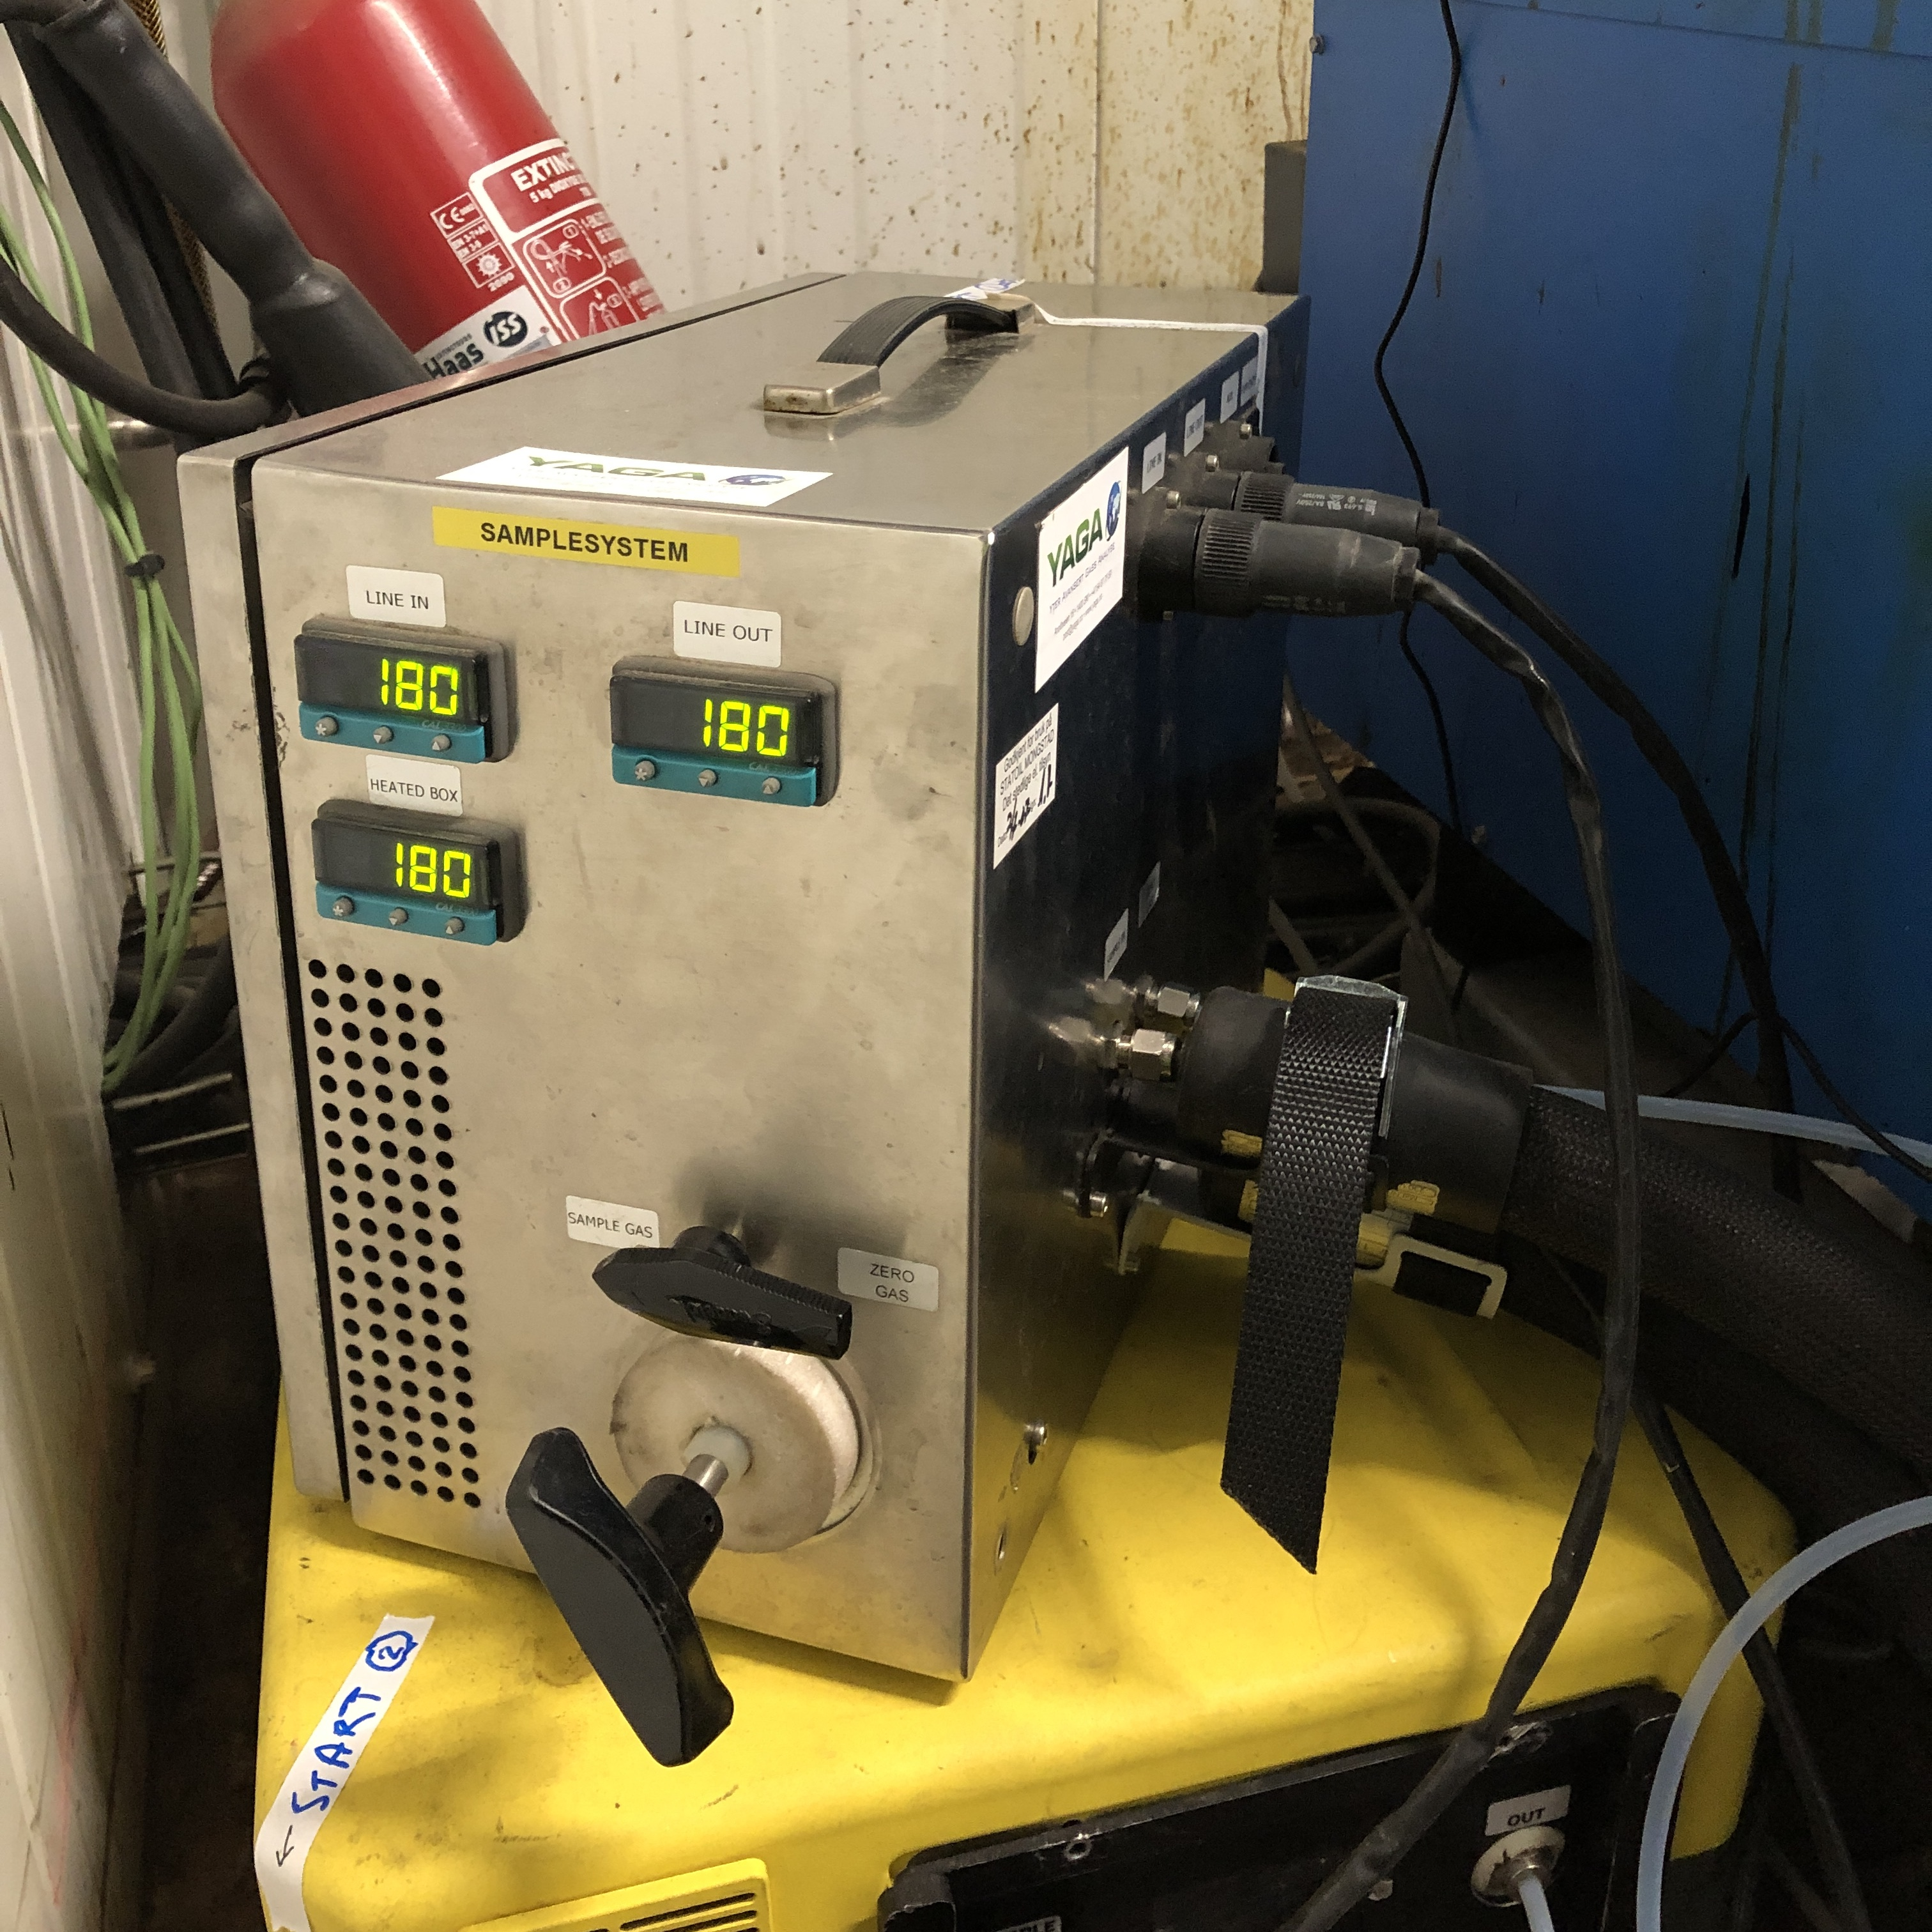
\includegraphics[width=0.6\textwidth]{Bilder/Pyrolysis/FTIR.jpg}
         \caption{}
         \label{appFig:FTIRbox}
     \end{subfigure}
     \hfill
     \begin{subfigure}[t]{\textwidth}
         \centering
         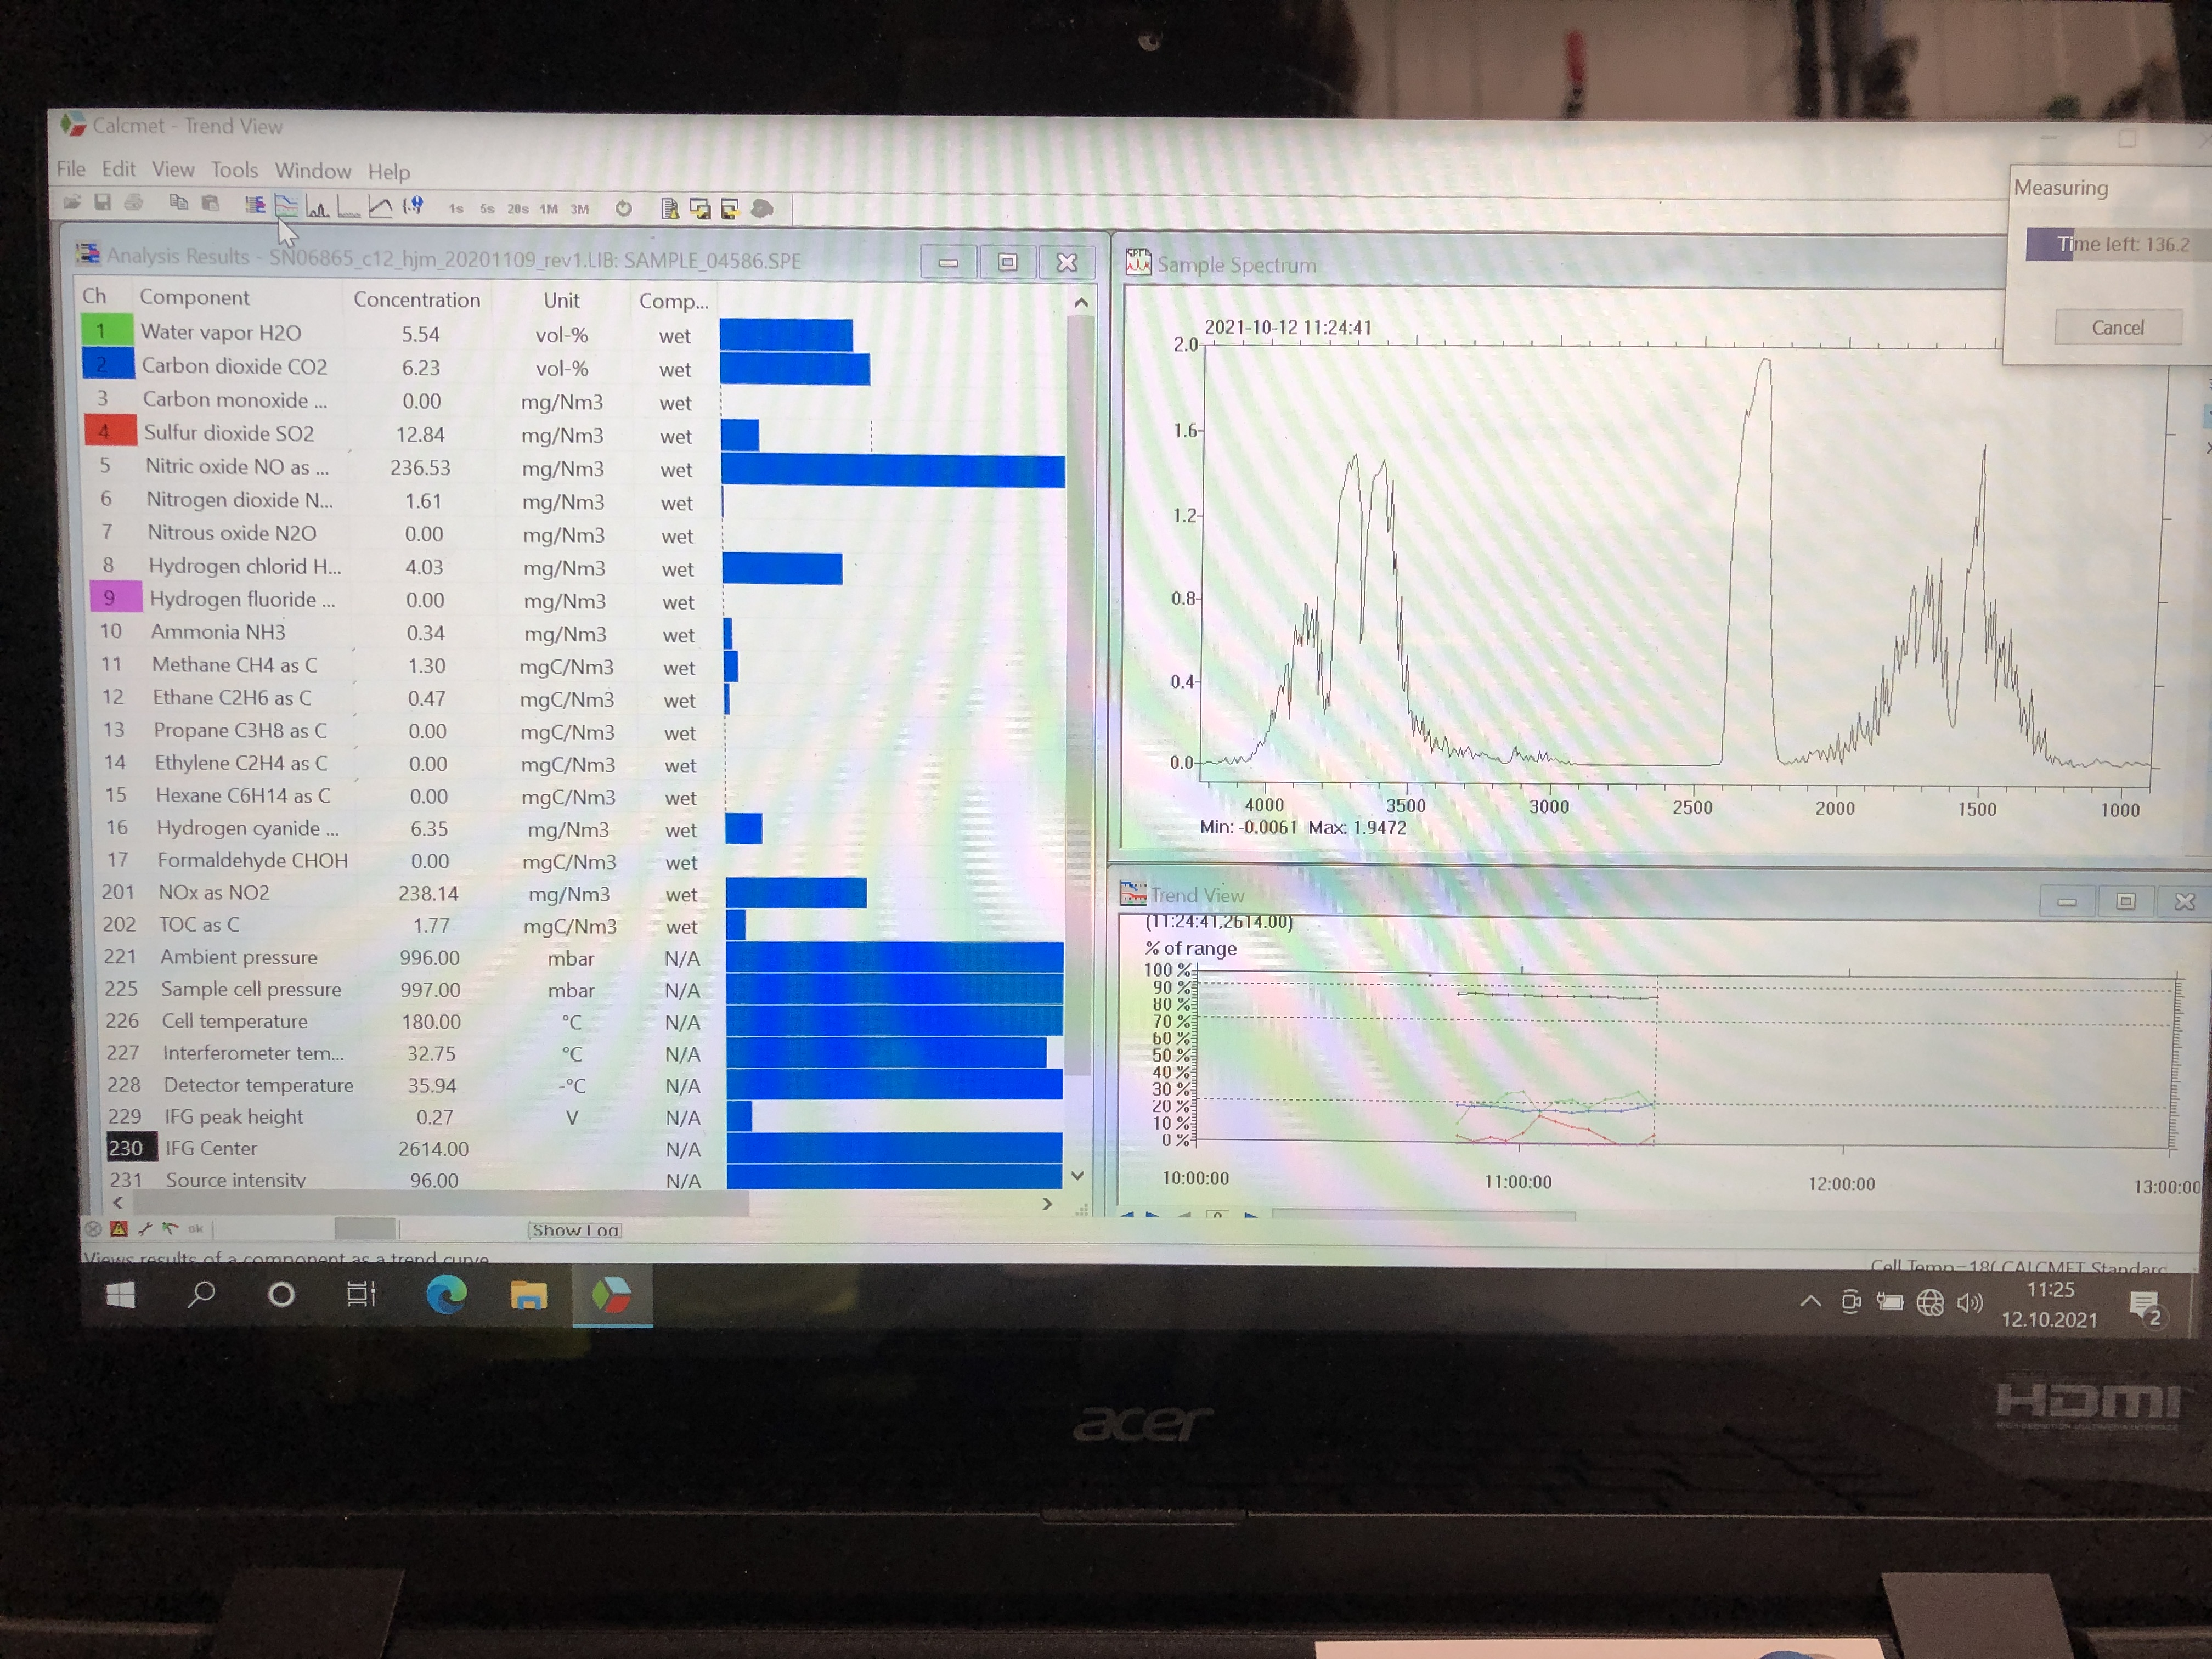
\includegraphics[width=0.6\textwidth]{Bilder/Pyrolysis/FTIRresults.png}
         \caption{}
         \label{appFig:FTIRresults}
     \end{subfigure}
     \hfill
     \caption{(a) FTIR. The tube leading to the FTIR is heated to 180 \textdegree C to prevent condensation of syn-gas. (b) FTIR output results. The results are a screenshot of the FTIR spectra from pyrolysis of Biorest Lindum (BRL).}
    \label{appFig:FTIR}
\end{figure}


\begin{figure}
    \centering
    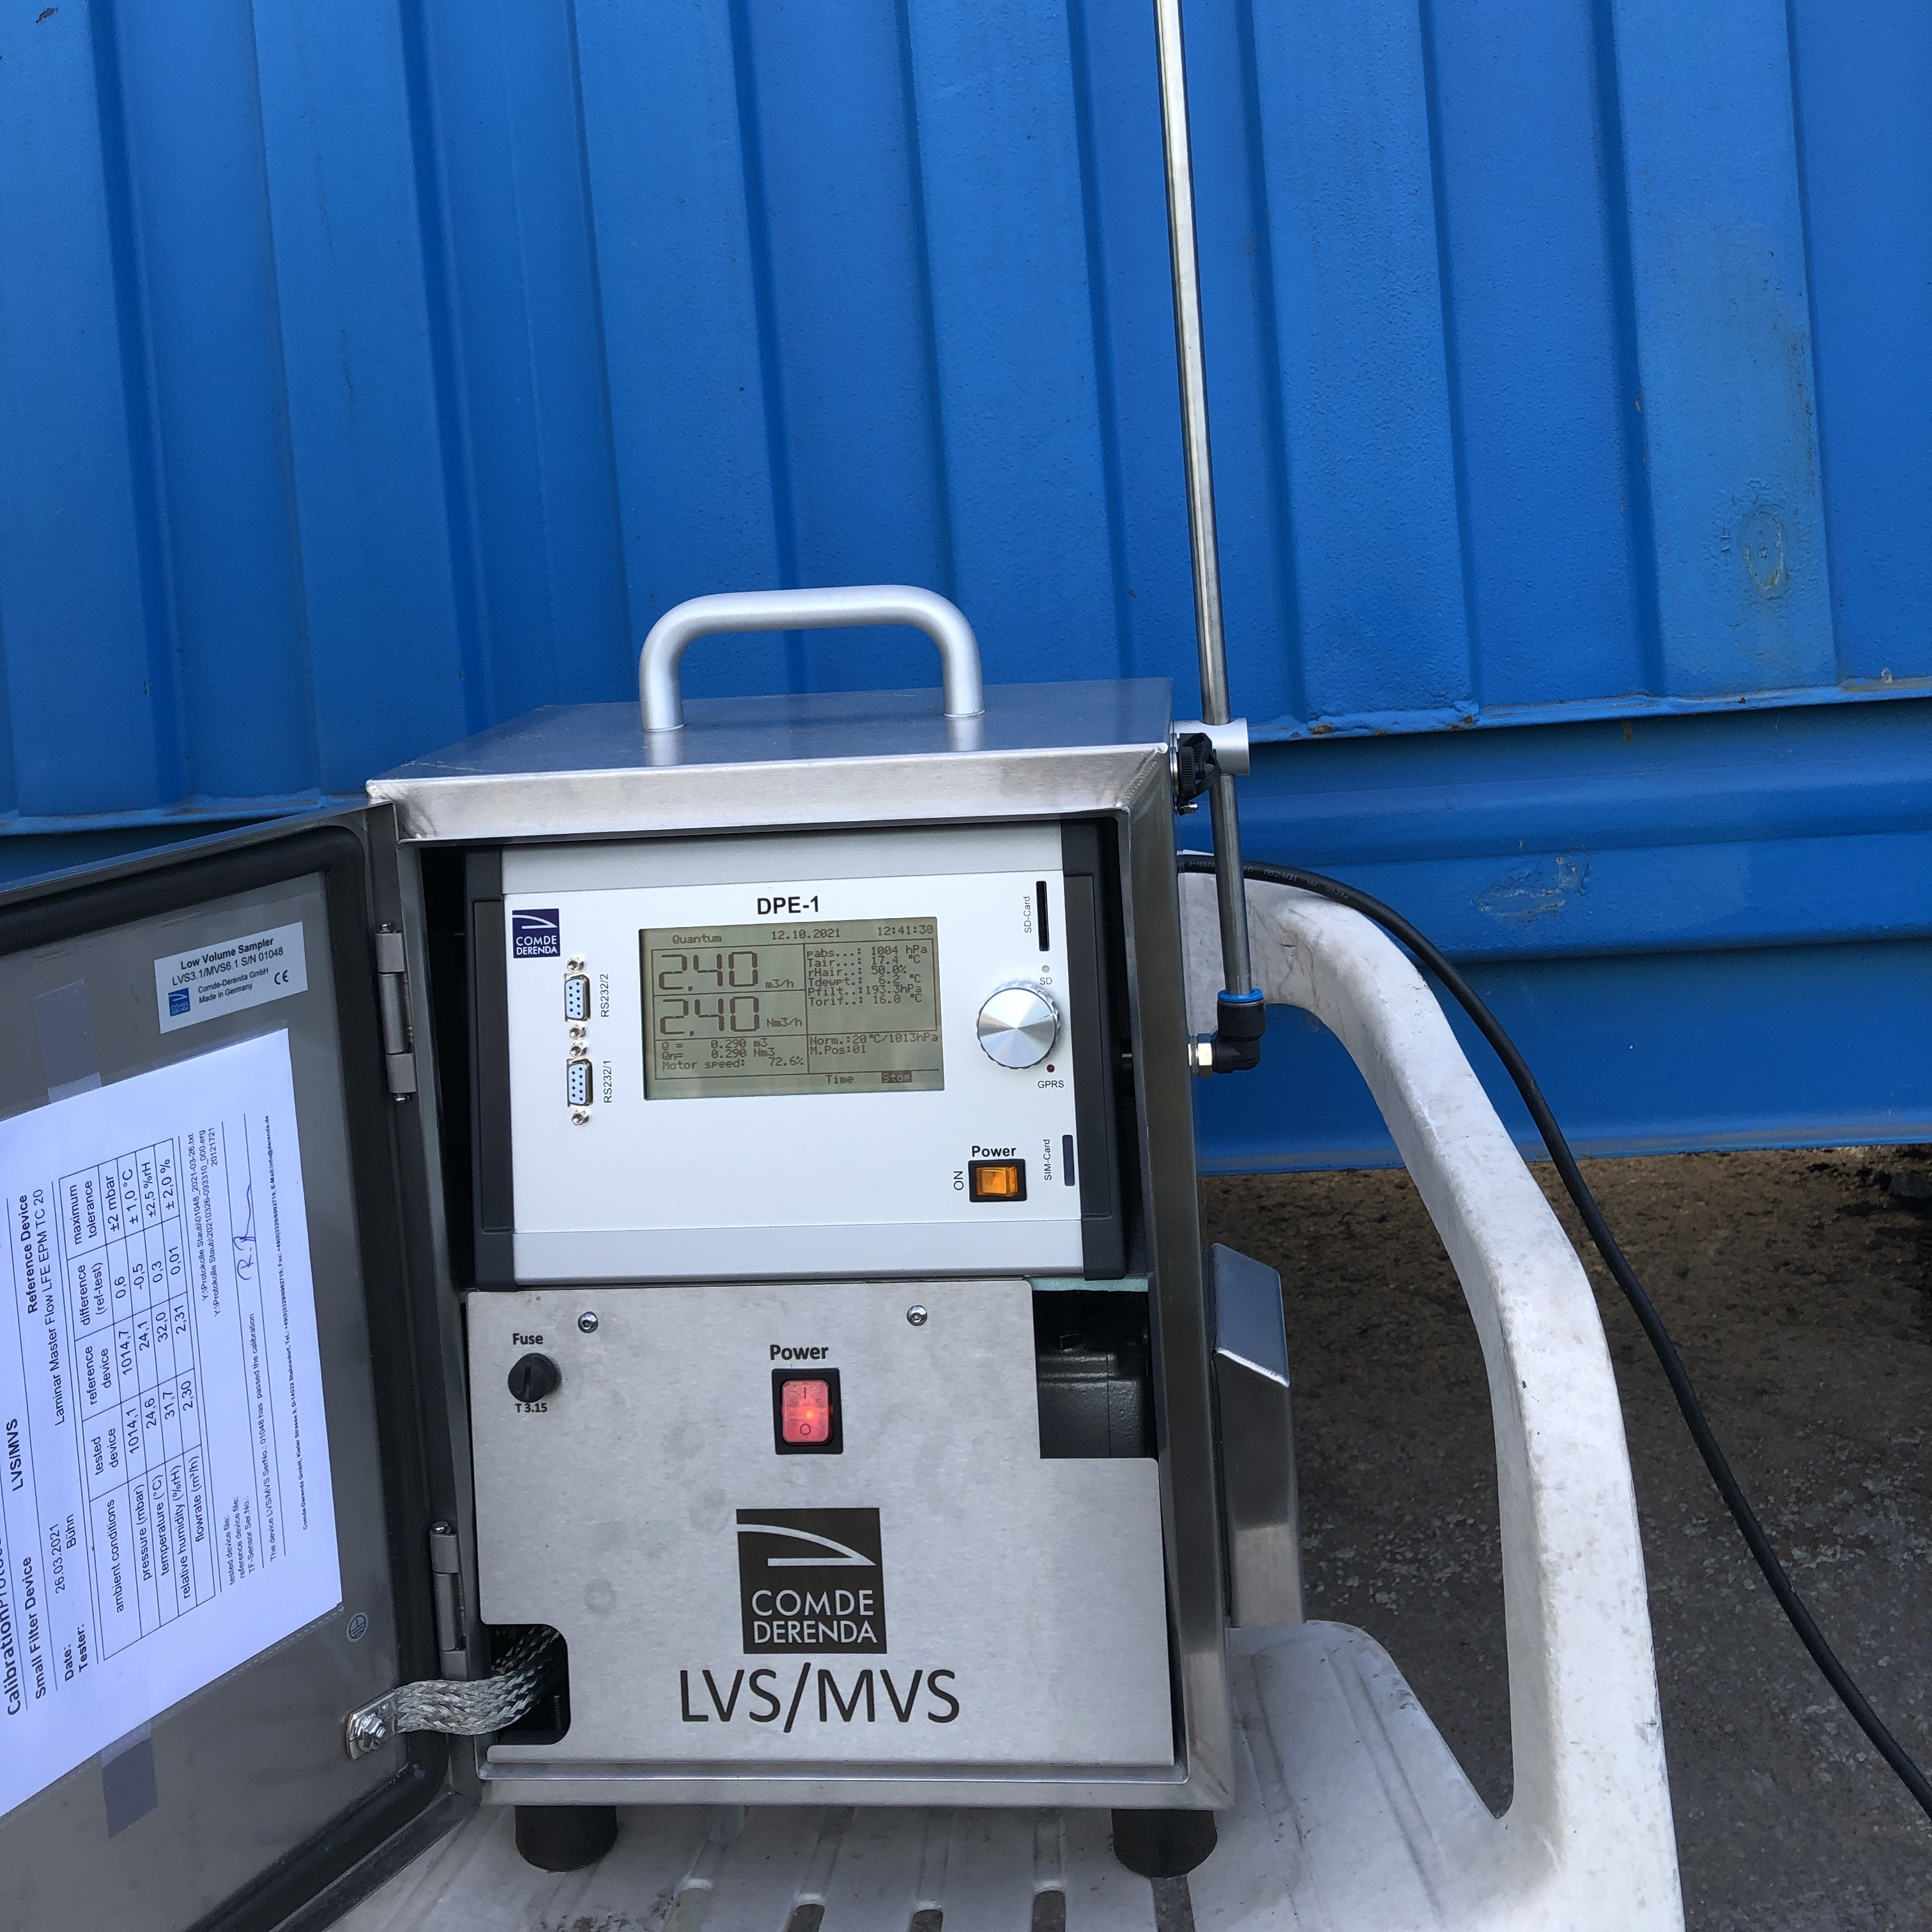
\includegraphics[width=0.85\textwidth]{Bilder/Pyrolysis/ParticlePump.jpg}
    \caption{LVS/MVS vacuum pump draws in air emitted from the ETIA chimney, and the sampler fractionates the airborne fine particles in a sampling inlet. The air containing the desired fine particulate fraction then passes through the filter, where the particles are collected and made available for subsequent gravimetric assessment or analysis. The volumetric flow rate is measured with an orifice plate and electronically adjusted with an accuracy of $\leq$ 2 $\%$. (Copied from comde-derenda.com, bust be rephrased)}
    \label{appFig:ParticlePump}
\end{figure}
